% Requires in the preamble:
% \usepackage{amsmath,amssymb}
% \usepackage{tikz,pgfplots}
% \pgfplotsset{compat=1.18}

\chapter{Limits and Continuity}
\label{chap:limits-continuity}

Chapter 2 ended with a small but important calculation.  For

\[
s(t)=t^2,
\]

the average velocity from \(t=2\) to \(t=2+h\) is

\[
\frac{s(2+h)-s(2)}{h}=4+h,
\qquad h\neq0.
\]

As \(h\) gets close to \(0\), this average velocity gets close to \(4\).  The value \(h=0\) is forbidden in the quotient, but we can move as close to it as we like.

That is the first shape of a limit:

\[
\text{the input approaches a value, and the output approaches a value.}
\]

The word ``approaches'' sounds informal.  This chapter turns it into mathematics.

\section{Limits from motion and approximation}
\label{sec:limits-motion-approximation}

A speedometer gives an instantaneous reading.  But if all we have is a position formula, we first see only average velocities over intervals.  The limit is the act of shrinking the interval until the average rate settles toward one number.

\subsection{Average velocity as the interval shrinks}
\label{subsec:average-velocity-shrinks}

Let

\[
s(t)=t^2
\]

be the position of an object moving along a line, measured in meters after \(t\) seconds.  We want the velocity at the instant \(t=2\).

Over the interval from \(2\) to \(2+h\), the average velocity is

\[
A(h)=\frac{s(2+h)-s(2)}{h},
\qquad h\neq0.
\]

Compute:

\[
A(h)
=
\frac{(2+h)^2-2^2}{h}
=
\frac{4+4h+h^2-4}{h}
=
\frac{4h+h^2}{h}.
\]

Since \(h\neq0\), we may divide by \(h\):

\[
A(h)=4+h.
\]

So the average velocity depends on the width \(h\) of the interval.

\[
\begin{array}{c|cccccc}
h & -0.1 & -0.01 & -0.001 & 0.001 & 0.01 & 0.1 \\ \hline
A(h)=4+h & 3.9 & 3.99 & 3.999 & 4.001 & 4.01 & 4.1
\end{array}
\]

The closer \(h\) is to \(0\), the closer \(A(h)\) is to \(4\).  This suggests that the instantaneous velocity at \(t=2\) should be

\[
4\text{ meters/second}.
\]

The important point is not only the answer.  The important point is how we got it:

\[
\text{instantaneous velocity}=\text{limit of average velocities.}
\]

\begin{figure}[h]
\centering
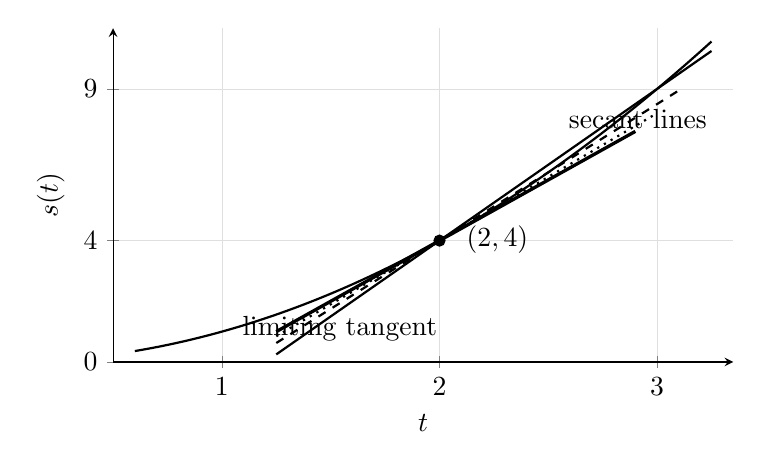
\begin{tikzpicture}
\begin{axis}[
    width=0.78\textwidth,
    height=0.48\textwidth,
    xmin=0.5, xmax=3.35,
    ymin=0, ymax=11,
    axis lines=left,
    xlabel={\(t\)},
    ylabel={\(s(t)\)},
    xtick={1,2,3},
    ytick={0,4,9},
    grid=both,
    grid style={line width=.1pt, draw=gray!25},
]
\addplot[thick, domain=0.6:3.25, samples=100] {x^2};
\addplot[thick, domain=1.25:3.25, samples=2] {5*x-6};
\addplot[thick, dashed, domain=1.25:3.1, samples=2] {4.5*x-5};
\addplot[thick, dotted, domain=1.25:3.0, samples=2] {4.2*x-4.4};
\addplot[very thick, domain=1.25:2.9, samples=2] {4*x-4};
\addplot[only marks, mark=*] coordinates {(2,4)};
\node[anchor=west] at (axis cs:2.08,4.05) {\((2,4)\)};
\node[anchor=west] at (axis cs:2.55,8.0) {secant lines};
\node[anchor=west] at (axis cs:1.05,1.1) {limiting tangent};
\end{axis}
\end{tikzpicture}
\caption{The slopes of the secant lines approach the slope of the tangent line at \(t=2\).}
\label{fig:secants-approach-tangent}
\end{figure}

The same calculation can be read geometrically.  The average velocity over an interval is the slope of a secant line.  As the second point moves toward \(t=2\), the secant line approaches a tangent line.

This is why limits are needed before derivatives can be defined.  A tangent slope is not usually found from two separated points.  It is found by letting one point approach another.

\subsection{Decimal approximations to a number}
\label{subsec:decimal-approximations-limit}

Limits do not belong only to motion.  They also appear whenever approximations close in on a target.

Chapter 2 used nested intervals to trap \(\sqrt2\):

\[
1.4<\sqrt2<1.5,
\]

\[
1.41<\sqrt2<1.42,
\]

\[
1.414<\sqrt2<1.415.
\]

The left endpoints

\[
1.4,\quad 1.41,\quad 1.414,\quad 1.4142,\quad \ldots
\]

approach \(\sqrt2\) from below.  The right endpoints approach it from above.  Neither finite list equals the whole number \(\sqrt2\), but the approximations can be made as close as desired.

A simpler example is

\[
1.9,\quad 1.99,\quad 1.999,\quad 1.9999,\quad \ldots
\]

These numbers approach \(2\).  The error after \(n\) decimal places is a power of \(10\):

\[
2-1.9=0.1,\qquad
2-1.99=0.01,\qquad
2-1.999=0.001.
\]

The errors approach \(0\).  So the approximations approach \(2\).

\begin{quote}
\textbf{A limit is a target value for a process.}

A number can be approached by decimal approximations.  A velocity can be approached by average velocities.  A tangent slope can be approached by secant slopes.
\end{quote}

The same idea appears in different clothing.  The mathematics is the same: errors are forced to become small.

\subsection{The informal meaning of a limit}
\label{subsec:informal-limit-meaning}

Let \(f\) be a function.  When we write

\[
\lim_{x\to a} f(x)=L,
\]

we mean:

\[
\text{as \(x\) gets close to \(a\), the values \(f(x)\) get close to \(L\).}
\]

The notation is read:

\[
\text{the limit of \(f(x)\) as \(x\) approaches \(a\) is \(L\).}
\]

There is one detail that must be said early:

\[
x\to a
\]

does not mean \(x=a\).  It means \(x\) is close to \(a\).  In many limits, the value at \(x=a\) is not used at all.

\begin{quote}
\textbf{Informal definition of a limit.}
We write

\[
\lim_{x\to a} f(x)=L
\]

if the values \(f(x)\) can be made as close to \(L\) as desired by taking \(x\) sufficiently close to \(a\), with \(x\neq a\).
\end{quote}

This definition is still informal because the phrases ``as close as desired'' and ``sufficiently close'' have not yet been made precise.  Section \ref{sec:precise-limit-definition} will do that.  For now, the informal definition is enough to compute and interpret many limits.

\paragraph{Example: a limit from a formula.}
Find

\[
\lim_{x\to 3}(2x+5).
\]

If \(x\) is close to \(3\), then \(2x+5\) is close to

\[
2(3)+5=11.
\]

So

\[
\lim_{x\to 3}(2x+5)=11.
\]

Here nothing strange happens at \(x=3\).  We can find the limit by direct substitution.

\paragraph{Example: the value at the point may not matter.}
Define

\[
F(x)=
\begin{cases}
2x+1, & x\neq1,\\
-1, & x=1.
\end{cases}
\]

Near \(x=1\), but not at \(x=1\), the function behaves like

\[
2x+1.
\]

As \(x\to1\),

\[
2x+1\to3.
\]

Therefore

\[
\lim_{x\to1}F(x)=3,
\]

even though

\[
F(1)=-1.
\]

\begin{figure}[h]
\centering
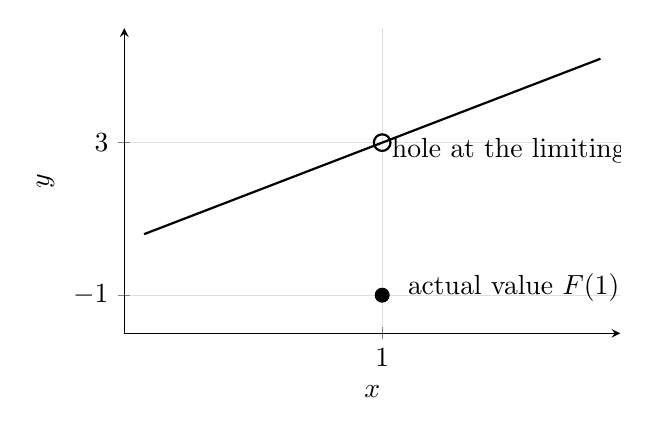
\begin{tikzpicture}
\begin{axis}[
    width=0.65\textwidth,
    height=0.45\textwidth,
    xmin=-0.3, xmax=2.2,
    ymin=-2, ymax=6,
    axis lines=left,
    xlabel={\(x\)},
    ylabel={\(y\)},
    xtick={1},
    ytick={-1,3},
    grid=both,
    grid style={line width=.1pt, draw=gray!25},
]
\addplot[thick, domain=-0.2:2.1, samples=2] {2*x+1};
\addplot[only marks, mark=o, mark size=3pt, thick] coordinates {(1,3)};
\addplot[only marks, mark=*, mark size=2.5pt] coordinates {(1,-1)};
\node[anchor=west] at (axis cs:1.0,2.8) {hole at the limiting value};
\node[anchor=west] at (axis cs:1.08,-0.8) {actual value \(F(1)\)};
\end{axis}
\end{tikzpicture}
\caption{The limit watches nearby values.  It does not have to equal the value of the function at the point.}
\label{fig:limit-hole-different-value}
\end{figure}

This example is important enough to remember:

\[
\boxed{\text{A limit near \(a\) is not the same thing as the value at \(a\).}}
\]

When the two do agree, we will have a special property called continuity.

\subsection{Limits from graphs and tables}
\label{subsec:limits-graphs-tables}

A graph can suggest a limit.  A table can suggest a limit.  But both must be read with care.

\paragraph{Example: a table that suggests a limit.}
Let

\[
g(x)=\frac{x^2-1}{x-1},
\qquad x\neq1.
\]

The formula is not defined at \(x=1\), but we can still examine values near \(1\).

\[
\begin{array}{c|cccccc}
x & 0.9 & 0.99 & 0.999 & 1.001 & 1.01 & 1.1 \\ \hline
g(x) & 1.9 & 1.99 & 1.999 & 2.001 & 2.01 & 2.1
\end{array}
\]

The values approach \(2\).  So the table suggests

\[
\lim_{x\to1}\frac{x^2-1}{x-1}=2.
\]

The table does not prove the limit.  It gives evidence.  Algebra will prove it in the next section.

\paragraph{Example: a graph that suggests no limit.}
Define

\[
J(x)=\frac{|x|}{x},
\qquad x\neq0.
\]

If \(x>0\), then \(|x|=x\), so

\[
J(x)=1.
\]

If \(x<0\), then \(|x|=-x\), so

\[
J(x)=-1.
\]

The values near \(0\) do not approach one common number.  From the right they stay at \(1\).  From the left they stay at \(-1\).

Therefore

\[
\lim_{x\to0}\frac{|x|}{x}
\]

does not exist.

\begin{figure}[h]
\centering
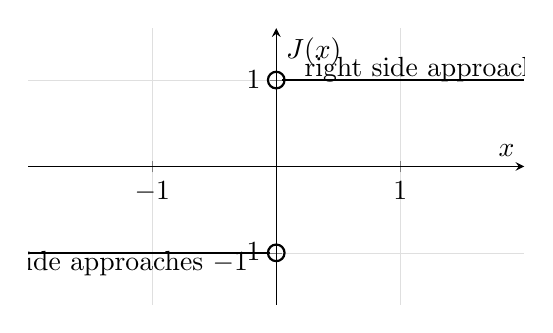
\begin{tikzpicture}
\begin{axis}[
    width=0.65\textwidth,
    height=0.42\textwidth,
    xmin=-2, xmax=2,
    ymin=-1.6, ymax=1.6,
    axis lines=middle,
    xlabel={\(x\)},
    ylabel={\(J(x)\)},
    xtick={-1,0,1},
    ytick={-1,1},
    grid=both,
    grid style={line width=.1pt, draw=gray!25},
]
\addplot[thick, domain=-2:-0.05, samples=2] {-1};
\addplot[thick, domain=0.05:2, samples=2] {1};
\addplot[only marks, mark=o, mark size=3pt, thick] coordinates {(0,-1) (0,1)};
\node[anchor=west] at (axis cs:0.15,1.12) {right side approaches \(1\)};
\node[anchor=east] at (axis cs:-0.15,-1.12) {left side approaches \(-1\)};
\end{axis}
\end{tikzpicture}
\caption{A two-sided limit exists only when nearby values approach one common target.}
\label{fig:jump-no-limit}
\end{figure}

The moral is simple:

\[
\boxed{\text{A limit must have one target.}}
\]

A jump gives two competing targets, so the two-sided limit does not exist.

\subsection{What a limit can ignore}
\label{subsec:what-limit-can-ignore}

The limit

\[
\lim_{x\to a}f(x)
\]

ignores the value \(f(a)\).  It watches what happens near \(a\).

That means all three situations below are possible.

\[
\begin{array}{c|c|c}
\textbf{situation} & \textbf{example} & \textbf{what happens} \\ \hline
f(a)\text{ exists and equals the limit} & f(x)=x^2,\ a=2 & \lim_{x\to2}f(x)=f(2)=4 \\[3pt]
f(a)\text{ exists but differs from the limit} &
F(x)=
\begin{cases}
2x+1,&x\neq1\\
-1,&x=1
\end{cases}
&
\lim_{x\to1}F(x)=3,\ F(1)=-1 \\[12pt]
f(a)\text{ does not exist, but the limit exists} &
g(x)=\dfrac{x^2-1}{x-1},\ a=1
&
\lim_{x\to1}g(x)=2
\end{array}
\]

The first situation is the calm one.  The second and third are warning signs.  They show why limits must come before continuity.

The next task is practical.  Graphs and tables help us guess limits, but calculus needs reliable ways to calculate them.  Algebra gives the first tools.

\section{Calculating limits}
\label{sec:calculating-limits}

A table can point toward a limit, but a table only checks a few inputs.  A graph can reveal the shape, but a graph depends on the viewing window.  Algebra lets us prove what the nearby values are doing.

The first limits we can calculate are the ones where nearby behavior is preserved by arithmetic.

\subsection{A first limit law from an example}
\label{subsec:first-limit-law-example}

Suppose

\[
f(x)=x^2
\qquad\text{and}\qquad
g(x)=3x-1.
\]

As \(x\to2\),

\[
f(x)\to4
\qquad\text{and}\qquad
g(x)\to5.
\]

Now look at their sum:

\[
f(x)+g(x)=x^2+3x-1.
\]

As \(x\to2\), this approaches

\[
4+5=9.
\]

So

\[
\lim_{x\to2}(x^2+3x-1)=9.
\]

The limit of the sum is the sum of the limits.

The same thing happens for products:

\[
f(x)g(x)=x^2(3x-1).
\]

As \(x\to2\), this approaches

\[
4\cdot5=20.
\]

So

\[
\lim_{x\to2}x^2(3x-1)=20.
\]

The nearby behavior of the pieces controls the nearby behavior of the expression built from them.

\subsection{Limit laws}
\label{subsec:limit-laws}

The example suggests the general rules.

\begin{quote}
\textbf{Limit laws.}
Suppose

\[
\lim_{x\to a}f(x)=L
\qquad\text{and}\qquad
\lim_{x\to a}g(x)=M.
\]

Then:

\[
\lim_{x\to a}\bigl(f(x)+g(x)\bigr)=L+M,
\]

\[
\lim_{x\to a}\bigl(f(x)-g(x)\bigr)=L-M,
\]

\[
\lim_{x\to a}\bigl(cf(x)\bigr)=cL
\qquad\text{for any constant }c,
\]

\[
\lim_{x\to a}\bigl(f(x)g(x)\bigr)=LM,
\]

and, if \(M\neq0\),

\[
\lim_{x\to a}\frac{f(x)}{g(x)}=\frac{L}{M}.
\]
\end{quote}

The condition \(M\neq0\) in the quotient law is not decoration.  Division by a quantity approaching \(0\) can behave wildly.

\paragraph{Why the sum law is believable.}
If \(f(x)\) is close to \(L\), and \(g(x)\) is close to \(M\), then

\[
f(x)+g(x)
\]

should be close to

\[
L+M.
\]

The error is controlled by

\[
\bigl|(f(x)+g(x))-(L+M)\bigr|
=
\bigl|(f(x)-L)+(g(x)-M)\bigr|.
\]

Using the triangle inequality,

\[
\bigl|(f(x)-L)+(g(x)-M)\bigr|
\le
|f(x)-L|+|g(x)-M|.
\]

So if both errors on the right are small, the error on the left is small.  This is the whole idea.  The precise \(\varepsilon\)-\(\delta\) proof will come later.

\paragraph{Warning: the quotient law needs a nonzero limiting denominator.}
Consider

\[
\frac{1}{x}.
\]

As \(x\to0\), the denominator approaches \(0\), and the quotient does not approach a finite number.  From the right it grows without bound; from the left it becomes negative without bound.

So we cannot use a quotient rule when the denominator limit is \(0\).  Sometimes a different algebraic simplification saves the limit.  Sometimes no finite limit exists.

\paragraph{Warning: limit laws do not work backward.}
It is possible for a sum to have a limit even when the pieces do not.

For \(x\neq0\), let

\[
f(x)=\sin\frac1x
\qquad\text{and}\qquad
g(x)=-\sin\frac1x.
\]

Neither \(f(x)\) nor \(g(x)\) approaches a single value as \(x\to0\).  They oscillate.  But

\[
f(x)+g(x)=0
\]

for every \(x\neq0\).  Therefore

\[
\lim_{x\to0}\bigl(f(x)+g(x)\bigr)=0.
\]

The limit law says:

\[
\text{if the two separate limits exist, then the limit of the sum is the sum.}
\]

It does not say the converse.

\subsection{Polynomials and direct substitution}
\label{subsec:polynomials-direct-substitution}

The limit laws immediately handle polynomials.

A polynomial is built from constants, powers of \(x\), sums, and products.  Since

\[
\lim_{x\to a}x=a,
\]

we get

\[
\lim_{x\to a}x^n=a^n
\]

for positive integers \(n\).  Then sums and constant multiples give the whole polynomial.

\begin{quote}
\textbf{Polynomial limit rule.}
If \(p(x)\) is a polynomial, then

\[
\lim_{x\to a}p(x)=p(a).
\]
\end{quote}

\paragraph{Example.}
Find

\[
\lim_{x\to -1}(3x^4-2x^2+5x-7).
\]

Because the expression is a polynomial, substitute \(x=-1\):

\[
3(-1)^4-2(-1)^2+5(-1)-7
=
3-2-5-7
=
-11.
\]

So

\[
\lim_{x\to -1}(3x^4-2x^2+5x-7)=-11.
\]

\subsection{Rational functions}
\label{subsec:rational-functions-limits}

A rational function is a quotient of polynomials:

\[
R(x)=\frac{p(x)}{q(x)}.
\]

If the denominator is not approaching \(0\), the quotient law applies.

\begin{quote}
\textbf{Rational function limit rule.}
If \(p\) and \(q\) are polynomials and \(q(a)\neq0\), then

\[
\lim_{x\to a}\frac{p(x)}{q(x)}
=
\frac{p(a)}{q(a)}.
\]
\end{quote}

\paragraph{Example.}
Find

\[
\lim_{x\to2}\frac{x^2+3x}{x-5}.
\]

The denominator at \(x=2\) is

\[
2-5=-3,
\]

which is not \(0\).  So direct substitution is legal:

\[
\lim_{x\to2}\frac{x^2+3x}{x-5}
=
\frac{2^2+3(2)}{2-5}
=
\frac{10}{-3}
=
-\frac{10}{3}.
\]

\paragraph{What direct substitution can tell us.}
When direct substitution gives a number, that number is the limit.

When direct substitution gives something like

\[
\frac{0}{0},
\]

it tells us only that the direct method failed.  It does not tell us the limit.  The expression may have a removable hole, or it may have no finite limit.

The next examples show the difference.

\subsection{Removing a removable discontinuity}
\label{subsec:removing-removable-discontinuity}

Return to

\[
g(x)=\frac{x^2-1}{x-1}.
\]

Direct substitution at \(x=1\) gives

\[
\frac{0}{0},
\]

so the rational function rule does not apply.

But the numerator factors:

\[
x^2-1=(x-1)(x+1).
\]

For \(x\neq1\),

\[
\frac{x^2-1}{x-1}
=
\frac{(x-1)(x+1)}{x-1}
=
x+1.
\]

When taking the limit as \(x\to1\), we are allowed to assume \(x\neq1\).  That is built into the meaning of a limit.  So near \(1\), except at \(1\), the function agrees with \(x+1\).

Therefore

\[
\lim_{x\to1}\frac{x^2-1}{x-1}
=
\lim_{x\to1}(x+1)
=
2.
\]

The original function has a hole at \(x=1\).  The simplified function fills the hole.

\begin{figure}[h]
\centering
\begin{tikzpicture}
\begin{axis}[
    width=0.65\textwidth,
    height=0.45\textwidth,
    xmin=-1.2, xmax=3,
    ymin=-0.5, ymax=4.5,
    axis lines=left,
    xlabel={\(x\)},
    ylabel={\(y\)},
    xtick={1},
    ytick={2},
    grid=both,
    grid style={line width=.1pt, draw=gray!25},
]
\addplot[thick, domain=-1:3, samples=2] {x+1};
\addplot[only marks, mark=o, mark size=3pt, thick] coordinates {(1,2)};
\node[anchor=west] at (axis cs:1.12,2.12) {hole};
\node[anchor=west] at (axis cs:1.7,2.65) {\(y=x+1\)};
\end{axis}
\end{tikzpicture}
\caption{For \(x\neq1\), \(\dfrac{x^2-1}{x-1}=x+1\).  The limit sees the nearby line, not the missing point.}
\label{fig:removable-hole}
\end{figure}

\paragraph{A second removable discontinuity.}
Find

\[
\lim_{x\to0}\frac{\sqrt{4+x}-2}{x}.
\]

Direct substitution gives

\[
\frac{0}{0}.
\]

The numerator contains a difference of square roots.  Multiply by the conjugate:

\[
\frac{\sqrt{4+x}-2}{x}
\cdot
\frac{\sqrt{4+x}+2}{\sqrt{4+x}+2}
=
\frac{(4+x)-4}{x(\sqrt{4+x}+2)}.
\]

So

\[
\frac{\sqrt{4+x}-2}{x}
=
\frac{x}{x(\sqrt{4+x}+2)}.
\]

For \(x\neq0\),

\[
\frac{\sqrt{4+x}-2}{x}
=
\frac{1}{\sqrt{4+x}+2}.
\]

Now the limit is easy:

\[
\lim_{x\to0}\frac{1}{\sqrt{4+x}+2}
=
\frac{1}{\sqrt4+2}
=
\frac14.
\]

Therefore

\[
\boxed{
\lim_{x\to0}\frac{\sqrt{4+x}-2}{x}
=
\frac14.
}
\]

This example also explains why algebraic rewriting matters in numerical work.  The original expression subtracts nearly equal numbers when \(x\) is small.  The rewritten expression avoids that subtraction.

\subsection{When cancellation does not save the limit}
\label{subsec:cancellation-does-not-save}

Not every \(\frac00\) expression has a removable hole.

Consider

\[
\frac{x}{x^2}.
\]

For \(x\neq0\),

\[
\frac{x}{x^2}=\frac1x.
\]

As \(x\to0\), this does not approach a finite number.  So

\[
\lim_{x\to0}\frac{x}{x^2}
\]

does not exist as a finite limit.

The symbol \(\frac00\) is called an \emph{indeterminate form}.  It means the expression needs more work.  It does not determine the answer.

\[
\begin{array}{c|c|c}
\textbf{limit} & \textbf{simplification} & \textbf{result} \\ \hline
\displaystyle \lim_{x\to1}\frac{x^2-1}{x-1}
&
x+1
&
2 \\[10pt]
\displaystyle \lim_{x\to0}\frac{x}{x^2}
&
\dfrac1x
&
\text{no finite two-sided limit}
\end{array}
\]

Same first appearance, different behavior.  This is why we do not treat \(\frac00\) as a number.

\subsection{The squeeze idea}
\label{subsec:squeeze-idea}

Some limits cannot be found by simplifying an expression into something calm.  Instead, we trap the function between two simpler functions.

Consider

\[
f(x)=x^2\sin\frac1x,
\qquad x\neq0.
\]

The factor \(\sin(1/x)\) oscillates faster and faster as \(x\to0\).  It does not approach any one number.  But it is always trapped between \(-1\) and \(1\):

\[
-1\le \sin\frac1x\le 1.
\]

Multiplying by \(x^2\), which is nonnegative, gives

\[
-x^2\le x^2\sin\frac1x\le x^2.
\]

As \(x\to0\),

\[
-x^2\to0
\qquad\text{and}\qquad
x^2\to0.
\]

The function is squeezed between two quantities that both approach \(0\).  Therefore it must also approach \(0\):

\[
\lim_{x\to0}x^2\sin\frac1x=0.
\]

\begin{figure}[h]
\centering
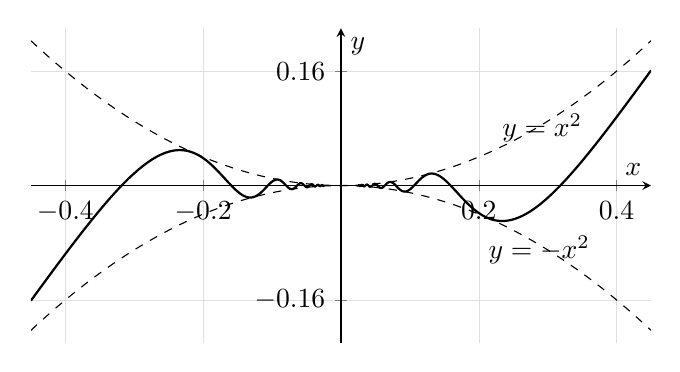
\begin{tikzpicture}
\begin{axis}[
    width=0.78\textwidth,
    height=0.46\textwidth,
    xmin=-0.45, xmax=0.45,
    ymin=-0.22, ymax=0.22,
    axis lines=middle,
    xlabel={\(x\)},
    ylabel={\(y\)},
    xtick={-0.4,-0.2,0.2,0.4},
    ytick={-0.16,0.16},
    grid=both,
    grid style={line width=.1pt, draw=gray!25},
]
\addplot[thick, domain=-0.45:-0.025, samples=500] {x^2*sin(deg(1/x))};
\addplot[thick, domain=0.025:0.45, samples=500] {x^2*sin(deg(1/x))};
\addplot[dashed, domain=-0.45:0.45, samples=100] {x^2};
\addplot[dashed, domain=-0.45:0.45, samples=100] {-x^2};
\node[anchor=west] at (axis cs:0.22,0.08) {\(y=x^2\)};
\node[anchor=west] at (axis cs:0.20,-0.09) {\(y=-x^2\)};
\end{axis}
\end{tikzpicture}
\caption{The oscillating graph is trapped between \(y=-x^2\) and \(y=x^2\).  The walls close in at \(0\).}
\label{fig:squeeze-x2-sin}
\end{figure}

\begin{quote}
\textbf{Squeeze Principle.}
Suppose that, for all \(x\) sufficiently close to \(a\) with \(x\neq a\),

\[
p(x)\le f(x)\le q(x).
\]

If

\[
\lim_{x\to a}p(x)=L
\qquad\text{and}\qquad
\lim_{x\to a}q(x)=L,
\]

then

\[
\lim_{x\to a}f(x)=L.
\]
\end{quote}

The squeeze principle is not a trick.  It is a statement about error.  If \(f(x)\) is trapped between two quantities that both get close to \(L\), then \(f(x)\) has no room to go anywhere else.

\paragraph{Why the two outside limits must match.}
The bounds must close in on the same number.  If all we know is

\[
-1\le \sin\frac1x\le1,
\]

then we cannot conclude that

\[
\sin\frac1x
\]

has a limit as \(x\to0\).  The walls \(-1\) and \(1\) do not close in.  In fact, \(\sin(1/x)\) has no limit at \(0\).

The squeeze principle works because the trap becomes narrow.

\subsection{A short guide to the first limit tools}
\label{subsec:first-limit-tools-guide}

The first questions to ask are these.

\[
\begin{array}{>{\centering\arraybackslash}p{0.35\textwidth}|p{0.56\textwidth}}
\textbf{what happens?} & \textbf{what to try} \\ \hline
direct substitution gives a number &
Use the polynomial or rational function rules. \\[4pt]
direct substitution gives \(\frac00\) &
Factor, cancel, expand, or rationalize.  Then try the limit again. \\[4pt]
an oscillating factor is multiplied by something small &
Try to squeeze it between two functions with the same limit. \\[4pt]
left and right behavior look different &
Do not force a two-sided limit.  The limit may fail to exist. \\[4pt]
the expression grows without bound &
A finite limit may not exist.  We will give this behavior a name soon.
\end{array}
\]

These tools are enough for many early limits.  They are not the whole story.  Limits can fail from a jump, explode toward infinity, or behave differently on the two sides of a point.

The next section separates those possibilities.  A limit can miss because the two sides disagree, or because the values do not settle down to any finite number.
\section{One-sided limits and infinite behavior}
\label{sec:one-sided-infinite-limits}

Section \ref{sec:calculating-limits} gave us tools for limits that settle down to a finite number.  But limits can fail, or change character, in several different ways.

A graph can approach one value from the left and another from the right.  A function can grow without bound near a point.  Or the input itself can move farther and farther away, so that we ask what happens at the far ends of the graph.

These are not rare exceptions.  They are some of the most important behaviors calculus has to name.

\subsection{Left-hand and right-hand limits}
\label{subsec:left-right-limits}

When we write

\[
x\to a,
\]

we usually mean that \(x\) approaches \(a\) from both sides.  But sometimes the two sides tell different stories.

Consider the function

\[
f(x)=
\begin{cases}
x+1, & x<2,\\
5, & x=2,\\
4-x, & x>2.
\end{cases}
\]

As \(x\) approaches \(2\) from the left, the values of \(f(x)\) follow the line

\[
y=x+1.
\]

So they approach

\[
2+1=3.
\]

As \(x\) approaches \(2\) from the right, the values of \(f(x)\) follow the line

\[
y=4-x.
\]

So they approach

\[
4-2=2.
\]

The value at the point is

\[
f(2)=5,
\]

but the value at the point is not what decides the nearby limit.

\begin{figure}[h]
\centering
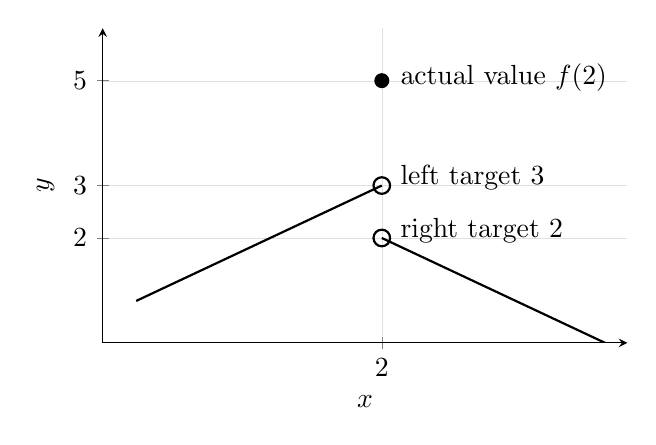
\begin{tikzpicture}
\begin{axis}[
    width=0.68\textwidth,
    height=0.46\textwidth,
    xmin=-0.5, xmax=4.2,
    ymin=0, ymax=6,
    axis lines=left,
    xlabel={\(x\)},
    ylabel={\(y\)},
    xtick={2},
    ytick={2,3,5},
    grid=both,
    grid style={line width=.1pt, draw=gray!25},
]
\addplot[thick, domain=-0.2:2, samples=2] {x+1};
\addplot[thick, domain=2:4, samples=2] {4-x};
\addplot[only marks, mark=o, mark size=3pt, thick] coordinates {(2,3) (2,2)};
\addplot[only marks, mark=*, mark size=2.5pt] coordinates {(2,5)};
\node[anchor=west] at (axis cs:2.08,3.15) {left target \(3\)};
\node[anchor=west] at (axis cs:2.08,2.15) {right target \(2\)};
\node[anchor=west] at (axis cs:2.08,5.05) {actual value \(f(2)\)};
\end{axis}
\end{tikzpicture}
\caption{The left and right sides approach different values.  Therefore the two-sided limit does not exist.}
\label{fig:one-sided-different-limits}
\end{figure}

We write

\[
\lim_{x\to2^-}f(x)=3.
\]

The symbol \(x\to2^-\) means that \(x\) approaches \(2\) from values less than \(2\).  This is called the \emph{left-hand limit}.

We write

\[
\lim_{x\to2^+}f(x)=2.
\]

The symbol \(x\to2^+\) means that \(x\) approaches \(2\) from values greater than \(2\).  This is called the \emph{right-hand limit}.

\begin{quote}
\textbf{One-sided limits.}

\[
\lim_{x\to a^-}f(x)=L
\]

means that \(f(x)\) approaches \(L\) as \(x\) approaches \(a\) from the left.

\[
\lim_{x\to a^+}f(x)=L
\]

means that \(f(x)\) approaches \(L\) as \(x\) approaches \(a\) from the right.
\end{quote}

The two-sided limit exists only when the two one-sided limits agree.

\begin{quote}
\textbf{Two-sided limit test.}
For a function defined near both sides of \(a\),

\[
\lim_{x\to a}f(x)=L
\]

if and only if

\[
\lim_{x\to a^-}f(x)=L
\qquad\text{and}\qquad
\lim_{x\to a^+}f(x)=L.
\]
\end{quote}

In the example above,

\[
\lim_{x\to2^-}f(x)=3,
\qquad
\lim_{x\to2^+}f(x)=2.
\]

Since

\[
3\neq2,
\]

the two-sided limit does not exist:

\[
\lim_{x\to2}f(x)\quad\text{does not exist.}
\]

\paragraph{Example: a removable hole has matching one-sided limits.}
Let

\[
g(x)=\frac{x^2-1}{x-1},
\qquad x\neq1.
\]

For \(x\neq1\),

\[
g(x)=x+1.
\]

Therefore

\[
\lim_{x\to1^-}g(x)=2
\qquad\text{and}\qquad
\lim_{x\to1^+}g(x)=2.
\]

The two one-sided limits agree, so

\[
\lim_{x\to1}g(x)=2.
\]

A missing value does not destroy a limit.  A jump usually does.

\paragraph{Example: absolute value divided by \(x\).}
For

\[
J(x)=\frac{|x|}{x},
\qquad x\neq0,
\]

we have

\[
J(x)=-1\quad\text{if }x<0,
\]

and

\[
J(x)=1\quad\text{if }x>0.
\]

Thus

\[
\lim_{x\to0^-}\frac{|x|}{x}=-1,
\qquad
\lim_{x\to0^+}\frac{|x|}{x}=1.
\]

The two-sided limit does not exist.

\[
\boxed{\text{A two-sided limit needs one common target.}}
\]

\subsection{Infinite limits and vertical asymptotes}
\label{subsec:infinite-limits-vertical-asymptotes}

A limit can fail in a different way.  The left and right sides might agree in direction, but the values might not settle near any finite number.

Consider

\[
f(x)=\frac{1}{(x-2)^2}.
\]

As \(x\) gets close to \(2\), the denominator

\[
(x-2)^2
\]

gets close to \(0\), but it remains positive.  Dividing \(1\) by a very small positive number gives a very large positive number.

\[
\begin{array}{c|cccccc}
x & 1.9 & 1.99 & 1.999 & 2.001 & 2.01 & 2.1 \\ \hline
\dfrac{1}{(x-2)^2} & 100 & 10{,}000 & 1{,}000{,}000
& 1{,}000{,}000 & 10{,}000 & 100
\end{array}
\]

The values do not approach a finite number.  They grow beyond any fixed bound.

We write

\[
\lim_{x\to2}\frac{1}{(x-2)^2}=\infty.
\]

This notation needs careful reading.  The symbol \(\infty\) is not a real number.  So this is not a finite limit.  It is a way of saying that the function grows without bound.

\begin{quote}
\textbf{Infinite limit, informally.}
We write

\[
\lim_{x\to a}f(x)=\infty
\]

if \(f(x)\) can be made larger than any chosen positive number by taking \(x\) sufficiently close to \(a\), with \(x\neq a\).
\end{quote}

Similarly,

\[
\lim_{x\to a}f(x)=-\infty
\]

means that \(f(x)\) becomes negative with arbitrarily large magnitude.

\paragraph{The sign matters.}
Now consider

\[
g(x)=\frac{1}{x-2}.
\]

If \(x>2\), then \(x-2>0\), so

\[
g(x)>0.
\]

As \(x\to2^+\), the denominator is a small positive number, so

\[
g(x)\to\infty.
\]

If \(x<2\), then \(x-2<0\), so

\[
g(x)<0.
\]

As \(x\to2^-\), the denominator is a small negative number, so

\[
g(x)\to-\infty.
\]

Thus

\[
\lim_{x\to2^-}\frac1{x-2}=-\infty,
\qquad
\lim_{x\to2^+}\frac1{x-2}=\infty.
\]

\begin{figure}[h]
\centering
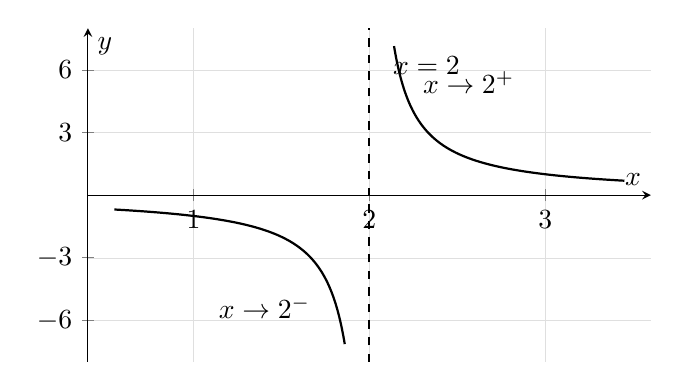
\begin{tikzpicture}
\begin{axis}[
    width=0.72\textwidth,
    height=0.48\textwidth,
    xmin=0.4, xmax=3.6,
    ymin=-8, ymax=8,
    axis lines=middle,
    xlabel={\(x\)},
    ylabel={\(y\)},
    xtick={1,2,3},
    ytick={-6,-3,3,6},
    grid=both,
    grid style={line width=.1pt, draw=gray!25},
]
\addplot[thick, domain=0.55:1.86, samples=160] {1/(x-2)};
\addplot[thick, domain=2.14:3.45, samples=160] {1/(x-2)};
\draw[dashed, thick] (axis cs:2,-8) -- (axis cs:2,8);
\node[anchor=west] at (axis cs:2.08,6.2) {\(x=2\)};
\node[anchor=east] at (axis cs:1.72,-5.4) {\(x\to2^-\)};
\node[anchor=west] at (axis cs:2.25,5.4) {\(x\to2^+\)};
\end{axis}
\end{tikzpicture}
\caption{The graph of \(1/(x-2)\) falls without bound from the left and rises without bound from the right.}
\label{fig:one-over-x-minus-two}
\end{figure}

The vertical line

\[
x=2
\]

is called a \emph{vertical asymptote}.

\begin{quote}
\textbf{Vertical asymptote.}
The line \(x=a\) is a vertical asymptote of the graph of \(f\) if at least one of the one-sided limits

\[
\lim_{x\to a^-}f(x),
\qquad
\lim_{x\to a^+}f(x)
\]

is \(\infty\) or \(-\infty\).
\end{quote}

A vertical asymptote often appears when a denominator approaches \(0\) and no cancellation removes the problem.

\paragraph{Example: cancellation versus asymptote.}
Compare

\[
\frac{x^2-1}{x-1}
\]

and

\[
\frac{x+1}{x-1}.
\]

For the first expression,

\[
x^2-1=(x-1)(x+1),
\]

so the factor \(x-1\) cancels for \(x\neq1\).  The graph has a hole, and

\[
\lim_{x\to1}\frac{x^2-1}{x-1}=2.
\]

For the second expression,

\[
\frac{x+1}{x-1},
\]

there is no cancellation.  As \(x\to1\), the numerator approaches \(2\), while the denominator approaches \(0\).  The function grows without bound in magnitude.

From the right,

\[
x-1>0,
\]

so

\[
\lim_{x\to1^+}\frac{x+1}{x-1}=\infty.
\]

From the left,

\[
x-1<0,
\]

so

\[
\lim_{x\to1^-}\frac{x+1}{x-1}=-\infty.
\]

Thus \(x=1\) is a vertical asymptote.

\[
\boxed{\frac00\text{ may hide a hole.}
\qquad
\frac{\text{nonzero}}0\text{ usually signals an asymptote.}}
\]

This is not a replacement for thought.  It is a warning about what to check.

\subsection{Limits at infinity}
\label{subsec:limits-at-infinity}

So far, the input \(x\) has approached a finite number.  But many questions ask what happens after a long time, far from the starting point, or for very large input.

For example, suppose the temperature of a cup of coffee in a room is modeled by

\[
T(t)=70+\frac{90}{t+1},
\qquad t\ge0,
\]

where \(T(t)\) is measured in degrees Fahrenheit and \(t\) is measured in hours.

At the start,

\[
T(0)=70+90=160.
\]

As \(t\) grows, the fraction

\[
\frac{90}{t+1}
\]

gets smaller.  The temperature approaches \(70\), the room temperature.

We write

\[
\lim_{t\to\infty}\left(70+\frac{90}{t+1}\right)=70.
\]

The notation \(t\to\infty\) does not mean that \(t\) approaches a number called infinity.  It means that \(t\) grows without bound.

\begin{quote}
\textbf{Limit at infinity, informally.}
We write

\[
\lim_{x\to\infty}f(x)=L
\]

if \(f(x)\) approaches \(L\) as \(x\) becomes arbitrarily large.

We write

\[
\lim_{x\to-\infty}f(x)=L
\]

if \(f(x)\) approaches \(L\) as \(x\) becomes negative with arbitrarily large magnitude.
\end{quote}

The basic limit behind many examples is

\[
\lim_{x\to\infty}\frac1x=0,
\qquad
\lim_{x\to-\infty}\frac1x=0.
\]

More generally, for any positive integer \(n\),

\[
\lim_{x\to\infty}\frac1{x^n}=0,
\qquad
\lim_{x\to-\infty}\frac1{x^n}=0.
\]

\paragraph{Example: rational function at infinity.}
Find

\[
\lim_{x\to\infty}\frac{3x^2-x+1}{x^2+4}.
\]

The highest power of \(x\) in the numerator and denominator is \(x^2\).  Divide every term by \(x^2\):

\[
\frac{3x^2-x+1}{x^2+4}
=
\frac{3-\frac1x+\frac1{x^2}}{1+\frac4{x^2}}.
\]

As \(x\to\infty\),

\[
\frac1x\to0
\qquad\text{and}\qquad
\frac1{x^2}\to0.
\]

Therefore

\[
\lim_{x\to\infty}\frac{3x^2-x+1}{x^2+4}
=
\frac{3-0+0}{1+0}
=
3.
\]

The same limit holds as \(x\to-\infty\):

\[
\lim_{x\to-\infty}\frac{3x^2-x+1}{x^2+4}=3.
\]

The largest powers control the far-away behavior.

\paragraph{A quick guide for rational functions.}
For a rational function

\[
R(x)=\frac{p(x)}{q(x)},
\]

the behavior as \(x\to\infty\) is controlled by the leading terms of \(p\) and \(q\).

\[
\begin{array}{c|c|c}
\textbf{degrees} & \textbf{example} & \textbf{behavior as }x\to\infty \\ \hline
\deg p<\deg q
&
\dfrac{x+1}{x^2+4}
&
0 \\[10pt]
\deg p=\deg q
&
\dfrac{3x^2-x+1}{x^2+4}
&
\dfrac{\text{leading coefficient of }p}{\text{leading coefficient of }q}=3 \\[12pt]
\deg p>\deg q
&
\dfrac{x^2+1}{x}
&
\text{does not approach a finite number}
\end{array}
\]

When the numerator has larger degree, the function may grow like a polynomial.  Sometimes it grows close to a line.  That leads to slant asymptotes.

\subsection{Horizontal and slant asymptotes}
\label{subsec:horizontal-slant-asymptotes}

A horizontal asymptote describes the far end of a graph.

\begin{quote}
\textbf{Horizontal asymptote.}
If

\[
\lim_{x\to\infty}f(x)=L
\]

or

\[
\lim_{x\to-\infty}f(x)=L,
\]

then the line

\[
y=L
\]

is a horizontal asymptote of the graph of \(f\) on that end.
\end{quote}

For the coffee model

\[
T(t)=70+\frac{90}{t+1},
\]

we have

\[
\lim_{t\to\infty}T(t)=70.
\]

So the graph has horizontal asymptote

\[
T=70.
\]

That asymptote has a physical meaning: it is the room temperature.

\paragraph{Different ends can have different horizontal asymptotes.}
Consider

\[
f(x)=\frac{x}{\sqrt{x^2+1}}.
\]

For \(x>0\),

\[
\sqrt{x^2+1}
=
x\sqrt{1+\frac1{x^2}},
\]

so

\[
f(x)=\frac{1}{\sqrt{1+\frac1{x^2}}}.
\]

Thus

\[
\lim_{x\to\infty}\frac{x}{\sqrt{x^2+1}}=1.
\]

For \(x<0\),

\[
\sqrt{x^2+1}
=
|x|\sqrt{1+\frac1{x^2}}
=
(-x)\sqrt{1+\frac1{x^2}}.
\]

So

\[
f(x)=
-\frac{1}{\sqrt{1+\frac1{x^2}}},
\]

and therefore

\[
\lim_{x\to-\infty}\frac{x}{\sqrt{x^2+1}}=-1.
\]

This graph has two different horizontal asymptotes:

\[
y=1
\quad\text{as }x\to\infty,
\]

and

\[
y=-1
\quad\text{as }x\to-\infty.
\]

\paragraph{Slant asymptotes.}
Some graphs do not approach a horizontal line.  Instead, they approach a tilted line.

Consider

\[
f(x)=\frac{x^2+1}{x-1}.
\]

Polynomial division gives

\[
x^2+1=(x-1)(x+1)+2.
\]

Therefore

\[
\frac{x^2+1}{x-1}
=
x+1+\frac{2}{x-1}.
\]

As \(x\to\infty\),

\[
\frac{2}{x-1}\to0.
\]

So

\[
f(x)-(x+1)\to0.
\]

The graph of \(f\) approaches the line

\[
y=x+1.
\]

That line is a \emph{slant asymptote}.

\begin{figure}[h]
\centering
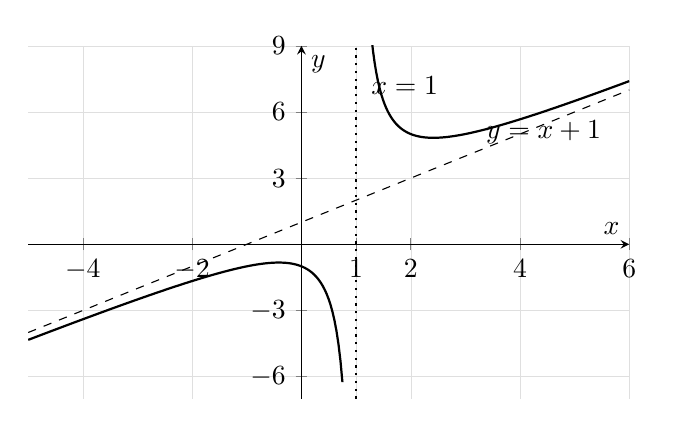
\begin{tikzpicture}
\begin{axis}[
    width=0.76\textwidth,
    height=0.50\textwidth,
    xmin=-5, xmax=6,
    ymin=-7, ymax=9,
    axis lines=middle,
    xlabel={\(x\)},
    ylabel={\(y\)},
    xtick={-4,-2,0,1,2,4,6},
    ytick={-6,-3,0,3,6,9},
    grid=both,
    grid style={line width=.1pt, draw=gray!25},
]
\addplot[thick, domain=-5:0.75, samples=160] {(x^2+1)/(x-1)};
\addplot[thick, domain=1.25:6, samples=160] {(x^2+1)/(x-1)};
\addplot[dashed, domain=-5:6, samples=2] {x+1};
\draw[dotted, thick] (axis cs:1,-7) -- (axis cs:1,9);
\node[anchor=west] at (axis cs:3.2,5.1) {\(y=x+1\)};
\node[anchor=west] at (axis cs:1.1,7.2) {\(x=1\)};
\end{axis}
\end{tikzpicture}
\caption{The graph of \(\dfrac{x^2+1}{x-1}\) has a vertical asymptote \(x=1\) and a slant asymptote \(y=x+1\).}
\label{fig:slant-asymptote}
\end{figure}

\begin{quote}
\textbf{Slant asymptote.}
The line

\[
y=mx+b,
\qquad m\neq0,
\]

is a slant asymptote of \(f\) as \(x\to\infty\) if

\[
\lim_{x\to\infty}\bigl(f(x)-(mx+b)\bigr)=0.
\]

The same definition applies as \(x\to-\infty\).
\end{quote}

The important quantity is not the ratio of \(f(x)\) to the line.  It is the vertical difference:

\[
f(x)-(mx+b).
\]

If that difference approaches \(0\), the graph approaches the line.

\subsection{A map of the new behaviors}
\label{subsec:map-new-limit-behaviors}

The word ``limit'' now covers several related ideas.

\[
\begin{array}{c|c|c}
\textbf{notation} & \textbf{input behavior} & \textbf{output behavior} \\ \hline
\displaystyle \lim_{x\to a}f(x)=L
&
x\text{ approaches }a\text{ from both sides}
&
f(x)\text{ approaches finite }L \\[6pt]
\displaystyle \lim_{x\to a^-}f(x)=L
&
x\text{ approaches }a\text{ from the left}
&
f(x)\text{ approaches finite }L \\[6pt]
\displaystyle \lim_{x\to a^+}f(x)=L
&
x\text{ approaches }a\text{ from the right}
&
f(x)\text{ approaches finite }L \\[6pt]
\displaystyle \lim_{x\to a}f(x)=\infty
&
x\text{ approaches }a
&
f(x)\text{ grows without bound} \\[6pt]
\displaystyle \lim_{x\to\infty}f(x)=L
&
x\text{ grows without bound}
&
f(x)\text{ approaches finite }L
\end{array}
\]

These ideas help us describe graphs accurately.  But the word ``approaches'' is still informal.  The next section turns it into a test that does not depend on the drawing or the table.

The test is based on a challenge: make the output error smaller than any tolerance I name.

\section{The precise definition of a limit}
\label{sec:precise-limit-definition}

The word ``approaches'' has done a lot of work.  It helped us describe average velocities, holes, jumps, asymptotes, and end behavior.  But pictures and tables can only suggest a limit.  To prove a limit, we need a precise test.

The test begins with error.

For \(s(t)=t^2\), the average velocity from \(t=2\) to \(t=2+h\) is

\[
A(h)=4+h,
\qquad h\neq0.
\]

We said that

\[
A(h)\to4
\qquad\text{as}\qquad
h\to0.
\]

Why?  Because the error is

\[
|A(h)-4|
=
|(4+h)-4|
=
|h|.
\]

If someone wants the output error to be less than \(0.01\), we can require

\[
|h|<0.01.
\]

If someone wants the output error to be less than \(0.000001\), we can require

\[
|h|<0.000001.
\]

Every requested output accuracy can be met by choosing a small enough input window around \(0\).

That is the whole idea of the precise definition.

\subsection{The epsilon challenge}
\label{subsec:epsilon-challenge}

The Greek letter \(\varepsilon\), pronounced ``epsilon,'' will represent the allowed output error.

To say that \(f(x)\) is within \(\varepsilon\) of \(L\) means

\[
|f(x)-L|<\varepsilon.
\]

This inequality says that \(f(x)\) lies in the interval

\[
(L-\varepsilon,L+\varepsilon).
\]

The number \(\varepsilon\) is not one special tiny number.  It means \emph{any} positive tolerance.

\[
\varepsilon=0.1,\quad
\varepsilon=0.001,\quad
\varepsilon=10^{-9}
\]

must all be allowed.

A limit claim must survive every epsilon challenge.

\begin{quote}
\textbf{The epsilon challenge.}
To prove

\[
\lim_{x\to a}f(x)=L,
\]

we must be able to make

\[
|f(x)-L|<\varepsilon
\]

for every \(\varepsilon>0\).
\end{quote}

The challenger chooses the output tolerance \(\varepsilon\).  We must respond by telling how close \(x\) must be to \(a\).

\subsection{Delta as a response}
\label{subsec:delta-response}

The Greek letter \(\delta\), pronounced ``delta,'' will represent the allowed input error.

To say that \(x\) is within \(\delta\) of \(a\), but not equal to \(a\), means

\[
0<|x-a|<\delta.
\]

The condition

\[
|x-a|<\delta
\]

places \(x\) inside the interval

\[
(a-\delta,a+\delta).
\]

The condition

\[
0<|x-a|
\]

removes the point \(x=a\).  This matters because a limit watches nearby values, not necessarily the value at the point.

Now we can state the definition.

\begin{quote}
\textbf{Precise definition of a finite limit.}
We write

\[
\lim_{x\to a}f(x)=L
\]

if the following condition holds:

For every \(\varepsilon>0\), there exists a \(\delta>0\) such that whenever \(x\) is in the domain of \(f\) and

\[
0<|x-a|<\delta,
\]

we have

\[
|f(x)-L|<\varepsilon.
\]
\end{quote}

The order matters.

\[
\boxed{
\text{First comes }\varepsilon.
\quad
\text{Then we choose }\delta.
}
\]

The value of \(\delta\) is allowed to depend on \(\varepsilon\).  Usually, smaller \(\varepsilon\) requires smaller \(\delta\).

\paragraph{The definition in one sentence.}
The limit of \(f(x)\) as \(x\to a\) is \(L\) if every output window around \(L\) contains all nearby values \(f(x)\), once \(x\) is restricted to a small enough punctured input window around \(a\).

\subsection{Why the point \(x=a\) is excluded}
\label{subsec:why-punctured}

The condition

\[
0<|x-a|
\]

is not a technical nuisance.  It preserves the meaning of a limit.

Recall the function

\[
F(x)=
\begin{cases}
2x+1, & x\neq1,\\
-1, & x=1.
\end{cases}
\]

We know that

\[
\lim_{x\to1}F(x)=3,
\]

even though

\[
F(1)=-1.
\]

If the definition forced us to check \(x=1\), then the output error from \(3\) would be

\[
|F(1)-3|=|-1-3|=4.
\]

For \(\varepsilon=1\), this would fail.  But that failure should not destroy the limit, because a limit is about nearby values.

The puncture

\[
0<|x-a|
\]

lets the limit ignore the value at \(a\).

\[
\boxed{\text{Limits are local around the point, not necessarily at the point.}}
\]

\subsection{Proving simple limits}
\label{subsec:proving-simple-limits}

An \(\varepsilon\)-\(\delta\) proof often begins by working backward.

We ask:

\[
\text{What condition on }|x-a|\text{ would force }|f(x)-L|<\varepsilon?
\]

Then we choose \(\delta\) to guarantee that condition.

\paragraph{Example: a linear function.}
Prove that

\[
\lim_{x\to3}(2x+5)=11.
\]

We need to make

\[
|(2x+5)-11|<\varepsilon.
\]

Simplify the error:

\[
|(2x+5)-11|
=
|2x-6|
=
2|x-3|.
\]

So it is enough to require

\[
2|x-3|<\varepsilon.
\]

That is,

\[
|x-3|<\frac{\varepsilon}{2}.
\]

This tells us what to choose:

\[
\delta=\frac{\varepsilon}{2}.
\]

\begin{quote}
\textbf{Proof.}
Let \(\varepsilon>0\) be given.  Choose

\[
\delta=\frac{\varepsilon}{2}.
\]

If

\[
0<|x-3|<\delta,
\]

then

\[
|(2x+5)-11|
=
2|x-3|
<
2\delta
=
2\cdot \frac{\varepsilon}{2}
=
\varepsilon.
\]

Therefore

\[
\lim_{x\to3}(2x+5)=11.
\]
\end{quote}

The proof does not say that \(x\) is close to \(3\) in vague language.  It gives a rule.  If the requested output error is \(\varepsilon\), then the input error \(\delta=\varepsilon/2\) is enough.

\paragraph{Example: a quadratic function.}
Prove that

\[
\lim_{x\to2}x^2=4.
\]

The output error is

\[
|x^2-4|.
\]

Factor:

\[
|x^2-4|
=
|x-2||x+2|.
\]

The factor \(|x-2|\) is the input error.  The other factor, \(|x+2|\), must be controlled.

If \(x\) is close to \(2\), then \(x+2\) is close to \(4\).  We only need a simple bound, not a perfect one.  Require

\[
|x-2|<1.
\]

Then

\[
1<x<3,
\]

so

\[
3<x+2<5.
\]

Thus

\[
|x+2|<5.
\]

Therefore, when \(|x-2|<1\),

\[
|x^2-4|
=
|x-2||x+2|
<
5|x-2|.
\]

To make this less than \(\varepsilon\), it is enough to require

\[
5|x-2|<\varepsilon,
\]

or

\[
|x-2|<\frac{\varepsilon}{5}.
\]

We need both requirements:

\[
|x-2|<1
\]

and

\[
|x-2|<\frac{\varepsilon}{5}.
\]

So choose the smaller of the two:

\[
\delta=\min\left(1,\frac{\varepsilon}{5}\right).
\]

\begin{quote}
\textbf{Proof.}
Let \(\varepsilon>0\) be given.  Choose

\[
\delta=\min\left(1,\frac{\varepsilon}{5}\right).
\]

If

\[
0<|x-2|<\delta,
\]

then \(|x-2|<1\), so

\[
|x+2|<5.
\]

Also,

\[
|x-2|<\frac{\varepsilon}{5}.
\]

Therefore

\[
|x^2-4|
=
|x-2||x+2|
<
5|x-2|
<
5\cdot \frac{\varepsilon}{5}
=
\varepsilon.
\]

Hence

\[
\lim_{x\to2}x^2=4.
\]
\end{quote}

This proof shows a common pattern.  We first restrict \(x\) to a simple neighborhood of \(a\) so that the extra factors stay bounded.  Then we choose a smaller \(\delta\) if needed to meet the desired error.

\paragraph{Example: a removable discontinuity.}
Prove that

\[
\lim_{x\to1}\frac{x^2-1}{x-1}=2.
\]

For \(x\neq1\),

\[
\frac{x^2-1}{x-1}
=
\frac{(x-1)(x+1)}{x-1}
=
x+1.
\]

The limit definition already assumes

\[
0<|x-1|,
\]

so \(x\neq1\).  Therefore the cancellation is legal for every \(x\) being tested.

The output error is

\[
\left|\frac{x^2-1}{x-1}-2\right|
=
|(x+1)-2|
=
|x-1|.
\]

So choose

\[
\delta=\varepsilon.
\]

\begin{quote}
\textbf{Proof.}
Let \(\varepsilon>0\) be given.  Choose

\[
\delta=\varepsilon.
\]

If

\[
0<|x-1|<\delta,
\]

then \(x\neq1\), and

\[
\left|\frac{x^2-1}{x-1}-2\right|
=
|x-1|
<
\delta
=
\varepsilon.
\]

Therefore

\[
\lim_{x\to1}\frac{x^2-1}{x-1}=2.
\]
\end{quote}

The hole at \(x=1\) causes no trouble.  The definition is built to ignore that point.

\subsection{Why the definition matches the picture}
\label{subsec:epsilon-delta-picture}

The picture behind the definition is simple.

Draw a horizontal band around the target value \(L\):

\[
L-\varepsilon<y<L+\varepsilon.
\]

The definition says that there must be a vertical strip around \(a\):

\[
a-\delta<x<a+\delta,
\qquad x\neq a,
\]

such that the graph inside that strip stays inside the horizontal band.

\begin{figure}[h]
\centering
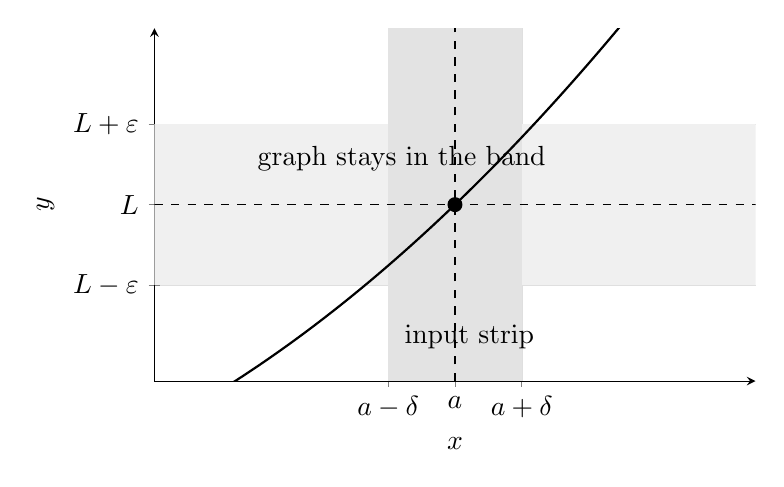
\begin{tikzpicture}
\begin{axis}[
    width=0.76\textwidth,
    height=0.50\textwidth,
    xmin=1.1, xmax=2.9,
    ymin=1.8, ymax=6.2,
    axis lines=left,
    xlabel={\(x\)},
    ylabel={\(y\)},
    xtick={1.8,2,2.2},
    xticklabels={\(a-\delta\),\(a\),\(a+\delta\)},
    ytick={3,4,5},
    yticklabels={\(L-\varepsilon\),\(L\),\(L+\varepsilon\)},
    grid=both,
    grid style={line width=.1pt, draw=gray!25},
]
\draw[fill=gray!12, draw=none] (axis cs:1.1,3) rectangle (axis cs:2.9,5);
\draw[fill=gray!22, draw=none] (axis cs:1.8,1.8) rectangle (axis cs:2.2,6.2);
\addplot[thick, domain=1.1:2.9, samples=120] {x^2};
\draw[dashed] (axis cs:2,1.8) -- (axis cs:2,6.2);
\draw[dashed] (axis cs:1.1,4) -- (axis cs:2.9,4);
\addplot[only marks, mark=*, mark size=2.5pt] coordinates {(2,4)};
\node[anchor=west] at (axis cs:1.38,4.57) {graph stays in the band};
\node[anchor=west] at (axis cs:1.82,2.35) {input strip};
\end{axis}
\end{tikzpicture}
\caption{For \(\lim_{x\to a}f(x)=L\), every horizontal band around \(L\) must contain the graph over some punctured vertical strip around \(a\).}
\label{fig:epsilon-delta-band-strip}
\end{figure}

There are two important details.

First, the horizontal band is chosen first.  That is the \(\varepsilon\)-challenge.

Second, the vertical strip may depend on the horizontal band.  A thinner output band usually requires a thinner input strip.

\paragraph{A failed two-sided limit.}
The definition also explains why

\[
\lim_{x\to0}\frac{|x|}{x}
\]

does not exist.

Suppose, for contradiction, that the limit were some number \(L\).  Choose

\[
\varepsilon=\frac12.
\]

No matter how small \(\delta>0\) is, both numbers

\[
x=\frac{\delta}{2}
\qquad\text{and}\qquad
x=-\frac{\delta}{2}
\]

satisfy

\[
0<|x|<\delta.
\]

But

\[
\frac{|\,\delta/2\,|}{\delta/2}=1,
\]

while

\[
\frac{|-\delta/2|}{-\delta/2}=-1.
\]

The definition would require both

\[
|1-L|<\frac12
\]

and

\[
|-1-L|<\frac12.
\]

The first inequality says

\[
\frac12<L<\frac32.
\]

The second says

\[
-\frac32<L<-\frac12.
\]

No number \(L\) can lie in both intervals.  Therefore no two-sided limit exists.

This is the precise version of the picture: the two sides approach different targets.

\subsection{One-sided versions of the precise definition}
\label{subsec:one-sided-precise-definition}

One-sided limits use the same idea, but the input is restricted to one side of the point.

For a left-hand limit,

\[
\lim_{x\to a^-}f(x)=L,
\]

the input condition becomes

\[
a-\delta<x<a.
\]

For a right-hand limit,

\[
\lim_{x\to a^+}f(x)=L,
\]

the input condition becomes

\[
a<x<a+\delta.
\]

The output condition remains the same:

\[
|f(x)-L|<\varepsilon.
\]

This is why the function

\[
J(x)=\frac{|x|}{x}
\]

has one-sided limits at \(0\).  From the left it is always \(-1\), and from the right it is always \(1\).  The one-sided tests pass separately, but the two-sided test fails because one \(\delta\)-window must handle both sides at once.

\subsection{What the definition gives us}
\label{subsec:what-epsilon-delta-gives}

The precise definition is not meant to replace intuition.  It protects intuition.

It explains why a table can suggest a limit but not prove it.  It explains why the value at the point may not matter.  It explains why a jump breaks a two-sided limit.  It gives us a way to prove limit laws instead of trusting them from graphs.

Most of the time, we will calculate limits using algebra, known limit laws, and continuity.  But the \(\varepsilon\)-\(\delta\) definition is the foundation underneath those shortcuts.

\begin{quote}
\textbf{What a finite limit really says.}
The statement

\[
\lim_{x\to a}f(x)=L
\]

means that output error can be forced below any chosen tolerance by making input error small enough, while not requiring \(x=a\).
\end{quote}

Now that limits have a precise meaning, we can define a special kind of well-behaved function.  It is the case where the nearby limit and the actual value agree.  That property is called continuity, and it is the reason many familiar graphs can be drawn without lifting the pencil.


\section{Continuity}
\label{sec:continuity}

The precise definition of a limit gave us a way to control nearby values.  It said:

\[
x\text{ close to }a
\quad \Longrightarrow \quad
f(x)\text{ close to }L.
\]

But a limit still does not have to care about the value at the point.  A function may have a hole, a wrong value, or no value at all, and still have a limit nearby.

Continuity is the calm case.  It is the case where the nearby behavior and the actual value agree.

\subsection{Continuity at a point}
\label{subsec:continuity-at-point}

Recall the function

\[
F(x)=
\begin{cases}
2x+1, & x\neq1,\\
-1, & x=1.
\end{cases}
\]

Near \(x=1\), but not at \(x=1\), the function follows the line

\[
y=2x+1.
\]

So

\[
\lim_{x\to1}F(x)=3.
\]

But

\[
F(1)=-1.
\]

The limit exists, but it does not equal the actual value.  The graph has the nearby behavior of the line \(y=2x+1\), except that the point at \(x=1\) has been placed somewhere else.

This function is not continuous at \(x=1\).

\begin{quote}
\textbf{Continuity at a point.}
A function \(f\) is \emph{continuous at \(a\)} if

\[
\lim_{x\to a}f(x)=f(a).
\]

Equivalently, three things must happen:

\[
\begin{array}{ll}
1. & f(a)\text{ is defined},\\
2. & \displaystyle \lim_{x\to a}f(x)\text{ exists},\\
3. & \displaystyle \lim_{x\to a}f(x)=f(a).
\end{array}
\]
\end{quote}

The third condition is the heart of the definition.  Nearby values must approach the actual value.

\[
\boxed{
\text{Continuity means: nearby inputs give nearby outputs, including at the point itself.}
}
\]

\paragraph{Example: a polynomial is continuous at a point.}
Let

\[
f(x)=x^2.
\]

At \(x=2\),

\[
f(2)=4.
\]

Also,

\[
\lim_{x\to2}x^2=4.
\]

Therefore

\[
\lim_{x\to2}f(x)=f(2),
\]

so \(f\) is continuous at \(2\).

In fact, the same reasoning works at every point.  If \(a\) is any real number, then

\[
\lim_{x\to a}x^2=a^2=f(a).
\]

So \(x^2\) is continuous everywhere.

\paragraph{The \(\varepsilon\)-\(\delta\) version.}
The limit definition gives a precise version of continuity.

A function \(f\) is continuous at \(a\) if, for every \(\varepsilon>0\), there is a \(\delta>0\) such that whenever \(x\) is in the domain of \(f\) and

\[
|x-a|<\delta,
\]

we have

\[
|f(x)-f(a)|<\varepsilon.
\]

There is no need to exclude \(x=a\) here.  If \(x=a\), then

\[
|f(x)-f(a)|=|f(a)-f(a)|=0,
\]

which is already less than every positive \(\varepsilon\).

So the limit definition uses a punctured interval:

\[
0<|x-a|<\delta,
\]

while continuity uses the full interval:

\[
|x-a|<\delta.
\]

\subsection{Holes and continuous extensions}
\label{subsec:holes-continuous-extensions}

Consider again

\[
g(x)=\frac{x^2-1}{x-1},
\qquad x\neq1.
\]

For \(x\neq1\),

\[
g(x)=x+1.
\]

Thus

\[
\lim_{x\to1}g(x)=2.
\]

But \(g(1)\) is not defined, because the original formula gives division by \(0\).  So \(g\) is not continuous at \(1\).

The failure is small.  The graph only has a missing point.  We can repair it by defining a new function

\[
\widetilde g(x)=
\begin{cases}
\dfrac{x^2-1}{x-1}, & x\neq1,\\[6pt]
2, & x=1.
\end{cases}
\]

Now

\[
\lim_{x\to1}\widetilde g(x)=2
\]

and

\[
\widetilde g(1)=2.
\]

Therefore \(\widetilde g\) is continuous at \(1\).

\begin{figure}[h]
\centering
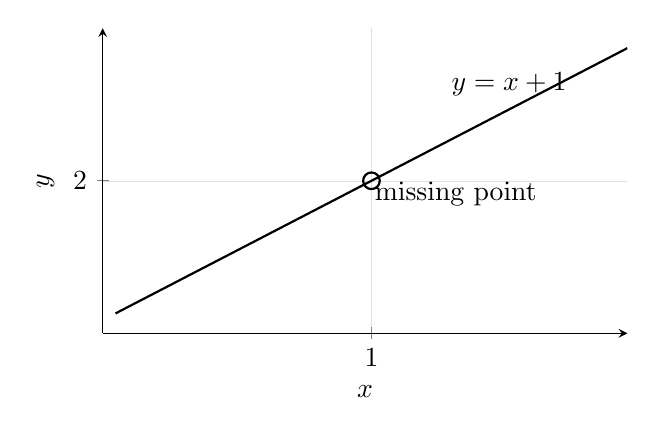
\begin{tikzpicture}
\begin{axis}[
    width=0.68\textwidth,
    height=0.45\textwidth,
    xmin=-1.1, xmax=3,
    ymin=-0.3, ymax=4.3,
    axis lines=left,
    xlabel={\(x\)},
    ylabel={\(y\)},
    xtick={1},
    ytick={2},
    grid=both,
    grid style={line width=.1pt, draw=gray!25},
]
\addplot[thick, domain=-1:3, samples=2] {x+1};
\addplot[only marks, mark=o, mark size=3pt, thick] coordinates {(1,2)};
\node[anchor=west] at (axis cs:0.95,1.8) {missing point};
\node[anchor=west] at (axis cs:1.55,3.45) {\(y=x+1\)};
\end{axis}
\end{tikzpicture}
\caption{The function \(\dfrac{x^2-1}{x-1}\) has the graph of \(y=x+1\), except for a missing point at \(x=1\).}
\label{fig:removable-continuity}
\end{figure}

A discontinuity like this is called \emph{removable}.  The limit tells us exactly what value to insert.

\begin{quote}
\textbf{Removable discontinuity.}
A function has a removable discontinuity at \(a\) if the limit

\[
\lim_{x\to a}f(x)
\]

exists, but the function is not continuous at \(a\) because \(f(a)\) is missing or has the wrong value.
\end{quote}

The word ``removable'' does not mean the original function was continuous.  It means we can make it continuous by changing the value at one point.

\subsection{Continuity on an interval}
\label{subsec:continuity-on-interval}

A function is continuous on an interval if it is continuous at every point of that interval.

For an open interval \((a,b)\), this means continuity at each point

\[
a<x<b.
\]

For a closed interval \([a,b]\), the endpoints need one-sided versions:

\[
\lim_{x\to a^+}f(x)=f(a)
\]

at the left endpoint, and

\[
\lim_{x\to b^-}f(x)=f(b)
\]

at the right endpoint.

\begin{quote}
\textbf{Continuity on a closed interval.}
A function \(f\) is continuous on \([a,b]\) if

\[
f\text{ is continuous at every point of }(a,b),
\]

\[
\lim_{x\to a^+}f(x)=f(a),
\]

and

\[
\lim_{x\to b^-}f(x)=f(b).
\]
\end{quote}

The one-sided conditions are natural.  At the left endpoint \(a\), points of the interval approach \(a\) only from the right.  At the right endpoint \(b\), points of the interval approach \(b\) only from the left.

\paragraph{Example: a piecewise function that is continuous.}
Define

\[
H(x)=
\begin{cases}
x^2, & x<1,\\
2x-1, & x\ge1.
\end{cases}
\]

Away from \(x=1\), each piece is a polynomial, so each piece is continuous.  The only point to check is \(x=1\).

From the left,

\[
\lim_{x\to1^-}H(x)=\lim_{x\to1^-}x^2=1.
\]

From the right,

\[
\lim_{x\to1^+}H(x)=\lim_{x\to1^+}(2x-1)=1.
\]

Also,

\[
H(1)=2(1)-1=1.
\]

Thus

\[
\lim_{x\to1}H(x)=H(1),
\]

so \(H\) is continuous at \(1\).  Therefore \(H\) is continuous everywhere.

\paragraph{Example: a piecewise function with a jump.}
Define

\[
J(x)=
\begin{cases}
x^2, & x<1,\\
2x, & x\ge1.
\end{cases}
\]

Again, the only point to check is \(x=1\).

From the left,

\[
\lim_{x\to1^-}J(x)=1.
\]

From the right,

\[
\lim_{x\to1^+}J(x)=2.
\]

The one-sided limits disagree, so

\[
\lim_{x\to1}J(x)
\]

does not exist.  Therefore \(J\) is not continuous at \(1\).

The formulas on the two sides are both harmless.  The problem is that they do not meet.

\subsection{Algebra of continuous functions}
\label{subsec:algebra-continuous-functions}

Continuity behaves well under the usual algebraic operations.  This is one reason continuous functions are easy to build.

Suppose \(f\) and \(g\) are continuous at \(a\).  Then

\[
f(x)\to f(a)
\qquad\text{and}\qquad
g(x)\to g(a)
\]

as \(x\to a\).  The limit laws give:

\[
f(x)+g(x)\to f(a)+g(a),
\]

\[
f(x)-g(x)\to f(a)-g(a),
\]

\[
f(x)g(x)\to f(a)g(a),
\]

and, if \(g(a)\neq0\),

\[
\frac{f(x)}{g(x)}\to \frac{f(a)}{g(a)}.
\]

So the new function is continuous at \(a\).

\begin{quote}
\textbf{Algebra of continuous functions.}
If \(f\) and \(g\) are continuous at \(a\), then the following functions are continuous at \(a\):

\[
f+g,\qquad f-g,\qquad cf,\qquad fg,
\]

where \(c\) is any constant.

If \(g(a)\neq0\), then

\[
\frac{f}{g}
\]

is also continuous at \(a\).
\end{quote}

The condition \(g(a)\neq0\) matters.  A quotient cannot be continuous at a point where its denominator is \(0\), because the quotient is not even defined there.

\paragraph{Example: a rational function.}
Let

\[
R(x)=\frac{x^2+3x+1}{x^2+1}.
\]

The numerator and denominator are polynomials, hence continuous everywhere.  The denominator satisfies

\[
x^2+1>0
\]

for every real \(x\).  Therefore \(R\) is continuous everywhere.

So, for example,

\[
\lim_{x\to2}\frac{x^2+3x+1}{x^2+1}
=
\frac{2^2+3(2)+1}{2^2+1}
=
\frac{11}{5}.
\]

Continuity is the reason direct substitution works here.

\paragraph{Basic continuous functions.}
The following functions are continuous at every point in their domains:

\[
\text{polynomials},
\]

\[
\text{rational functions where the denominator is not zero},
\]

\[
\sin x,\quad \cos x,\quad \tan x\text{ where defined},
\]

\[
e^x,\quad a^x\text{ for }a>0,
\]

\[
\ln x\text{ for }x>0,
\]

and root functions where they are defined.

This fact does not make limits disappear.  It gives us a shortcut when no hole, jump, or asymptote is present.

\subsection{Continuity of compositions}
\label{subsec:continuity-compositions}

Algebra builds new functions by adding, multiplying, and dividing.  Composition builds new functions by putting one function inside another.

Suppose

\[
g(x)\to g(a)
\]

as \(x\to a\), and suppose \(f\) is continuous at \(g(a)\).  Then

\[
f(g(x))\to f(g(a)).
\]

That is exactly the continuity of \(f\circ g\) at \(a\).

\begin{quote}
\textbf{Continuity of compositions.}
If \(g\) is continuous at \(a\), and \(f\) is continuous at \(g(a)\), then

\[
f\circ g
\]

is continuous at \(a\).  In symbols,

\[
\lim_{x\to a}f(g(x))=f(g(a)).
\]
\end{quote}

The order of the statement matters.  First \(g(x)\) must approach \(g(a)\).  Then \(f\) must preserve that approach near the input \(g(a)\).

\paragraph{Example.}
The function

\[
q(x)=\sqrt{1+x^2}
\]

is continuous for every real \(x\).  The inside function

\[
g(x)=1+x^2
\]

is continuous everywhere.  Its values are always at least \(1\), so the square root is defined.  Since the square root function is continuous on \([0,\infty)\), the composition is continuous everywhere.

Therefore

\[
\lim_{x\to3}\sqrt{1+x^2}
=
\sqrt{1+3^2}
=
\sqrt{10}.
\]

\paragraph{Example.}
The function

\[
r(x)=\sin(x^2)
\]

is continuous everywhere because \(x^2\) is continuous everywhere and sine is continuous everywhere.  Thus

\[
\lim_{x\to a}\sin(x^2)=\sin(a^2).
\]

This kind of substitution is legal because continuity protects it.

\subsection{Three common discontinuities}
\label{subsec:three-common-discontinuities}

Continuity can fail in several ways.  The three most common early failures are removable discontinuities, jump discontinuities, and infinite discontinuities.

\[
\begin{array}{c|c|c}
\textbf{type} & \textbf{what happens} & \textbf{example} \\ \hline
\text{removable} &
\text{limit exists, but value is missing or wrong}
&
\displaystyle \frac{x^2-1}{x-1}\text{ at }x=1 \\[10pt]
\text{jump} &
\text{left and right limits disagree}
&
\displaystyle \frac{|x|}{x}\text{ at }x=0 \\[10pt]
\text{infinite} &
\text{values grow without bound}
&
\displaystyle \frac{1}{(x-2)^2}\text{ at }x=2
\end{array}
\]

\begin{figure}[h]
\centering
\begin{minipage}{0.31\textwidth}
\centering
\begin{tikzpicture}
\begin{axis}[
    width=\textwidth,
    height=0.88\textwidth,
    xmin=-0.5, xmax=2.5,
    ymin=0, ymax=4,
    axis lines=middle,
    xtick={1},
    ytick={2},
    title={removable},
    grid=both,
    grid style={line width=.1pt, draw=gray!25},
]
\addplot[thick, domain=-0.2:2.3, samples=2] {x+1};
\addplot[only marks, mark=o, mark size=2.8pt, thick] coordinates {(1,2)};
\end{axis}
\end{tikzpicture}
\end{minipage}
\hfill
\begin{minipage}{0.31\textwidth}
\centering
\begin{tikzpicture}
\begin{axis}[
    width=\textwidth,
    height=0.88\textwidth,
    xmin=-2, xmax=2,
    ymin=-1.6, ymax=1.6,
    axis lines=middle,
    xtick={0},
    ytick={-1,1},
    title={jump},
    grid=both,
    grid style={line width=.1pt, draw=gray!25},
]
\addplot[thick, domain=-2:-0.05, samples=2] {-1};
\addplot[thick, domain=0.05:2, samples=2] {1};
\addplot[only marks, mark=o, mark size=2.8pt, thick] coordinates {(0,-1) (0,1)};
\end{axis}
\end{tikzpicture}
\end{minipage}
\hfill
\begin{minipage}{0.31\textwidth}
\centering
\begin{tikzpicture}
\begin{axis}[
    width=\textwidth,
    height=0.88\textwidth,
    xmin=0.2, xmax=3.8,
    ymin=0, ymax=8,
    axis lines=middle,
    xtick={2},
    ytick={4},
    title={infinite},
    grid=both,
    grid style={line width=.1pt, draw=gray!25},
]
\addplot[thick, domain=0.55:1.65, samples=120] {1/(x-2)^2};
\addplot[thick, domain=2.35:3.45, samples=120] {1/(x-2)^2};
\draw[dashed, thick] (axis cs:2,0) -- (axis cs:2,8);
\end{axis}
\end{tikzpicture}
\end{minipage}
\caption{Three common ways continuity can fail: a hole, a jump, or a vertical asymptote.}
\label{fig:three-discontinuities}
\end{figure}

The names are not just vocabulary.  They tell us what kind of repair, if any, is possible.

A removable discontinuity can be fixed by changing one value.

A jump cannot be fixed by changing one value, because the two sides approach different targets.

An infinite discontinuity cannot be fixed by changing one value, because nearby values do not stay near any finite number.

\subsection{A continuity checklist}
\label{subsec:continuity-checklist}

When checking continuity at \(a\), ask:

\[
\begin{array}{c|p{0.58\textwidth}}
\textbf{question} & \textbf{meaning} \\ \hline
\text{Is }f(a)\text{ defined?} &
If not, the function is not continuous at \(a\). \\[4pt]
\text{Does }\lim_{x\to a}f(x)\text{ exist?} &
If the two sides disagree or the values do not settle, the function is not continuous at \(a\). \\[4pt]
\text{Does the limit equal }f(a)\text{?} &
If not, the nearby behavior and the actual value disagree.
\end{array}
\]

For familiar formulas, continuity often lets us substitute directly.  For piecewise functions, endpoints between pieces must be checked.  For quotients, denominators must be watched.  For roots and logarithms, the domain must be respected.

Continuity is still a local idea: it describes what happens near one point.  But it has surprising global consequences.  A continuous graph cannot jump over a height, and on a closed finite interval it cannot avoid having a highest and lowest point.

Those two facts are the next payoff.

\section{Two theorems about continuous functions}
\label{sec:two-theorems-continuous-functions}

Continuity began as a local condition:

\[
x\text{ close to }a
\quad \Longrightarrow \quad
f(x)\text{ close to }f(a).
\]

But local calm forces global behavior.  If a continuous graph starts below a horizontal line and ends above it, it must cross that line somewhere.  If a continuous graph lives on a closed finite interval, it must reach a highest point and a lowest point.

These facts sound obvious from a picture.  Their hypotheses are where the mathematics lives.

\subsection{Intermediate values}
\label{subsec:intermediate-values}

Suppose the temperature outside is \(50^\circ\)F at sunrise and \(74^\circ\)F at noon.  If the temperature changes continuously, then at some time between sunrise and noon it must have been \(60^\circ\)F.

It cannot move from \(50\) to \(74\) without passing through the values in between.

The same idea solves equations.

\paragraph{Example: finding a root without a formula.}
Let

\[
p(x)=x^3-x-1.
\]

Then

\[
p(1)=1-1-1=-1
\]

and

\[
p(2)=8-2-1=5.
\]

The value of \(p(x)\) changes from negative to positive on the interval \([1,2]\).  Since \(p\) is a polynomial, it is continuous.  Therefore the graph must cross the \(x\)-axis somewhere between \(1\) and \(2\).

So there is a number \(c\in(1,2)\) such that

\[
p(c)=0.
\]

In other words,

\[
c^3-c-1=0.
\]

We have proved that the equation has a solution in \((1,2)\), even though we have not found an exact formula for \(c\).

\begin{figure}[h]
\centering
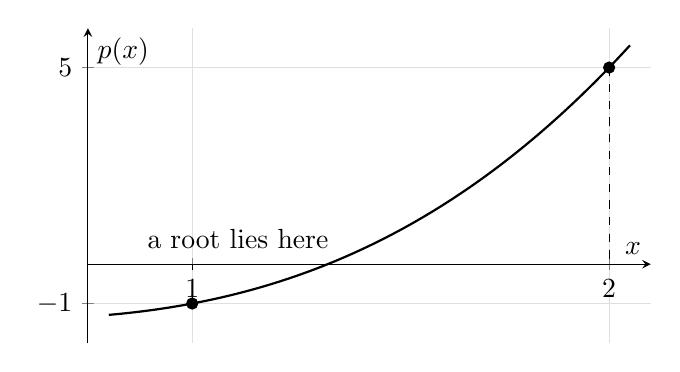
\begin{tikzpicture}
\begin{axis}[
    width=0.72\textwidth,
    height=0.46\textwidth,
    xmin=0.75, xmax=2.1,
    ymin=-2, ymax=6,
    axis lines=middle,
    xlabel={\(x\)},
    ylabel={\(p(x)\)},
    xtick={1,2},
    ytick={-1,0,5},
    grid=both,
    grid style={line width=.1pt, draw=gray!25},
]
\addplot[thick, domain=0.8:2.05, samples=120] {x^3-x-1};
\addplot[only marks, mark=*] coordinates {(1,-1) (2,5)};
\draw[dashed] (axis cs:1,-1) -- (axis cs:1,0);
\draw[dashed] (axis cs:2,5) -- (axis cs:2,0);
\node[anchor=south east] at (axis cs:1.35,0.15) {a root lies here};
\end{axis}
\end{tikzpicture}
\caption{A continuous graph that goes from negative to positive must cross the \(x\)-axis.}
\label{fig:ivt-root-cubic}
\end{figure}

This example is the Intermediate Value Theorem in miniature.

\begin{quote}
\textbf{Intermediate Value Theorem.}
Suppose \(f\) is continuous on the closed interval \([a,b]\).  If \(N\) is any number between \(f(a)\) and \(f(b)\), then there is at least one number \(c\in[a,b]\) such that

\[
f(c)=N.
\]
\end{quote}

If

\[
f(a)<N<f(b),
\]

then the theorem says that \(f\) hits the value \(N\) somewhere between \(a\) and \(b\).  The same is true if

\[
f(b)<N<f(a).
\]

The graph may wiggle many times.  It may hit the value \(N\) more than once.  The theorem promises at least one hit, not exactly one.

\paragraph{Root form of the theorem.}
A common special case is \(N=0\).

If \(f\) is continuous on \([a,b]\) and

\[
f(a)<0<f(b),
\]

or

\[
f(b)<0<f(a),
\]

then there is a number \(c\in(a,b)\) such that

\[
f(c)=0.
\]

This is the form used to prove that equations have solutions.

\subsection{Bisection as a constructive proof idea}
\label{subsec:bisection-proof-idea}

The Intermediate Value Theorem says a solution exists.  Bisection shows how to trap one.

Return to

\[
p(x)=x^3-x-1.
\]

We know

\[
p(1)<0
\qquad\text{and}\qquad
p(2)>0.
\]

Start with the interval

\[
[1,2].
\]

Cut it in half.  The midpoint is

\[
1.5.
\]

Compute:

\[
p(1.5)=1.5^3-1.5-1=0.875>0.
\]

So a sign change occurs on

\[
[1,1.5],
\]

because

\[
p(1)<0
\qquad\text{and}\qquad
p(1.5)>0.
\]

Cut again.  The midpoint of \([1,1.5]\) is

\[
1.25.
\]

Compute:

\[
p(1.25)=1.25^3-1.25-1=-0.296875<0.
\]

So a sign change occurs on

\[
[1.25,1.5].
\]

Continuing this process traps a root in smaller and smaller intervals.

\[
\begin{array}{c|c|c|c}
\textbf{step} & \textbf{interval} & \textbf{midpoint} & \textbf{sign at midpoint} \\ \hline
0 & [1,2] & 1.5 & + \\[2pt]
1 & [1,1.5] & 1.25 & - \\[2pt]
2 & [1.25,1.5] & 1.375 & + \\[2pt]
3 & [1.25,1.375] & 1.3125 & -
\end{array}
\]

After each step, the interval is half as long as before.  The intervals are nested:

\[
[1,2]\supset[1,1.5]\supset[1.25,1.5]\supset[1.25,1.375]\supset\cdots.
\]

The Nested Interval Principle traps one real number \(c\) in all these intervals.  Continuity then forces

\[
p(c)=0.
\]

\begin{quote}
\textbf{Idea of the proof of the Intermediate Value Theorem.}
For a target value \(N\), apply bisection to

\[
h(x)=f(x)-N.
\]

If \(h(a)\) and \(h(b)\) have opposite signs, repeatedly keep the half interval where the sign change remains.  The nested intervals shrink to a point \(c\).  Continuity prevents \(h(c)\) from being positive or negative, so

\[
h(c)=0.
\]

Therefore

\[
f(c)=N.
\]
\end{quote}

This proof idea shows why the real line matters.  Bisection produces smaller and smaller intervals.  The real numbers guarantee that the intervals trap an actual point.

\paragraph{What the theorem does not say.}
The Intermediate Value Theorem guarantees existence, not a formula.  It tells us a root exists in \((1,2)\), but it does not tell us the exact root.

Bisection gives approximations.  If we keep cutting long enough, we can make the interval around the root as short as desired.  This is one of the first reliable numerical methods in calculus.

\subsection{Why continuity is required}
\label{subsec:ivt-continuity-required}

The Intermediate Value Theorem fails without continuity.

Define

\[
S(x)=
\begin{cases}
0, & x<0,\\
2, & x\ge0.
\end{cases}
\]

On the interval \([-1,1]\),

\[
S(-1)=0
\qquad\text{and}\qquad
S(1)=2.
\]

The number \(1\) lies between \(0\) and \(2\).  But there is no \(c\in[-1,1]\) such that

\[
S(c)=1.
\]

The function jumps from \(0\) to \(2\).  It never takes the intermediate value \(1\).

\begin{figure}[h]
\centering
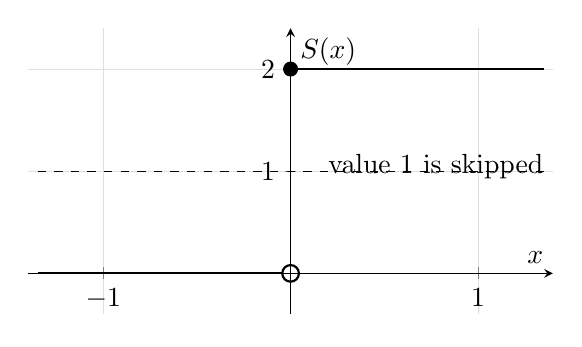
\begin{tikzpicture}
\begin{axis}[
    width=0.68\textwidth,
    height=0.43\textwidth,
    xmin=-1.4, xmax=1.4,
    ymin=-0.4, ymax=2.4,
    axis lines=middle,
    xlabel={\(x\)},
    ylabel={\(S(x)\)},
    xtick={-1,0,1},
    ytick={0,1,2},
    grid=both,
    grid style={line width=.1pt, draw=gray!25},
]
\addplot[thick, domain=-1.35:-0.04, samples=2] {0};
\addplot[thick, domain=0:1.35, samples=2] {2};
\addplot[only marks, mark=o, mark size=3pt, thick] coordinates {(0,0)};
\addplot[only marks, mark=*, mark size=2.5pt] coordinates {(0,2)};
\draw[dashed] (axis cs:-1.35,1) -- (axis cs:1.35,1);
\node[anchor=west] at (axis cs:0.15,1.05) {value \(1\) is skipped};
\end{axis}
\end{tikzpicture}
\caption{Without continuity, a graph can jump over an intermediate value.}
\label{fig:ivt-fails-jump}
\end{figure}

The hypothesis of continuity is not decoration.  It prevents jumping.

\subsection{Highest and lowest values}
\label{subsec:highest-lowest-values}

Continuity also gives a second global promise.

Suppose \(h(t)\) gives the height of a hiker above sea level at time \(t\), for \(0\le t\le4\).  If \(h\) is continuous, then during those four hours the hiker reaches a highest elevation and a lowest elevation.

The hiker cannot have a ``least upper bound'' of heights that is approached but never reached, as long as the time interval includes its endpoints and is finite.

A simple graph shows the idea.

Let

\[
f(x)=x(2-x)
\]

on the interval \([0,2]\).  This function is continuous.  Its values include

\[
f(0)=0,
\qquad
f(1)=1,
\qquad
f(2)=0.
\]

The absolute maximum value is

\[
1,
\]

attained at

\[
x=1.
\]

The absolute minimum value is

\[
0,
\]

attained at the endpoints

\[
x=0
\qquad\text{and}\qquad
x=2.
\]

\begin{figure}[h]
\centering
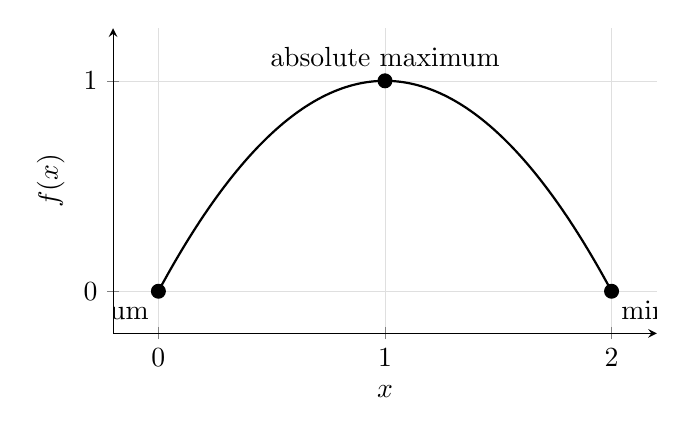
\begin{tikzpicture}
\begin{axis}[
    width=0.70\textwidth,
    height=0.45\textwidth,
    xmin=-0.2, xmax=2.2,
    ymin=-0.2, ymax=1.25,
    axis lines=left,
    xlabel={\(x\)},
    ylabel={\(f(x)\)},
    xtick={0,1,2},
    ytick={0,1},
    grid=both,
    grid style={line width=.1pt, draw=gray!25},
]
\addplot[thick, domain=0:2, samples=120] {x*(2-x)};
\addplot[only marks, mark=*, mark size=2.5pt] coordinates {(0,0) (1,1) (2,0)};
\node[anchor=south] at (axis cs:1,1.02) {absolute maximum};
\node[anchor=north east] at (axis cs:0,0) {minimum};
\node[anchor=north west] at (axis cs:2,0) {minimum};
\end{axis}
\end{tikzpicture}
\caption{A continuous function on a closed finite interval reaches its highest and lowest values.}
\label{fig:evt-parabola}
\end{figure}

The theorem says this always happens.

\begin{quote}
\textbf{Extreme Value Theorem.}
If \(f\) is continuous on a closed interval \([a,b]\), then \(f\) attains an absolute maximum and an absolute minimum on \([a,b]\).

That is, there are numbers \(c,d\in[a,b]\) such that

\[
f(c)\le f(x)\le f(d)
\]

for every \(x\in[a,b]\).
\end{quote}

The number \(f(d)\) is the absolute maximum value.  The number \(f(c)\) is the absolute minimum value.

The theorem does not say where the maximum and minimum occur.  They may occur at interior points, at endpoints, or at several points.

\paragraph{Example.}
The function

\[
f(x)=x^3-3x
\]

is continuous on \([-2,2]\), so the Extreme Value Theorem guarantees an absolute maximum and an absolute minimum on \([-2,2]\).

We do not yet have the derivative tools to find them efficiently.  But we already know they exist.

This is how the theorem will be used later.  Before optimizing a continuous function on a closed interval, we know that the best and worst values are really there.

\subsection{Why closed and bounded intervals matter}
\label{subsec:closed-bounded-matter}

The Extreme Value Theorem has two interval hypotheses:

\[
[a,b]\text{ is closed}
\qquad\text{and}\qquad
[a,b]\text{ is bounded}.
\]

Both matter.

\paragraph{If the interval is not closed.}
Consider

\[
f(x)=x
\]

on the open interval

\[
(0,1).
\]

The values of \(f\) get close to \(1\), but never equal \(1\), because \(x=1\) is not in the interval.  So \(f\) has no absolute maximum on \((0,1)\).

The values also get close to \(0\), but never equal \(0\), because \(x=0\) is not in the interval.  So \(f\) has no absolute minimum on \((0,1)\).

The missing endpoints matter.

\paragraph{If the interval is not bounded.}
Consider

\[
f(x)=x
\]

on the whole real line

\[
(-\infty,\infty).
\]

There is no largest value and no smallest value.  The function can grow as large as we like and as negative as we like.

The function is continuous, but the interval is unbounded.  The conclusion fails.

\paragraph{If the function is not continuous.}
Even on a closed bounded interval, discontinuity can break the conclusion.

Define

\[
K(x)=
\begin{cases}
x, & 0\le x<1,\\
0, & x=1.
\end{cases}
\]

The domain is the closed interval \([0,1]\), but \(K\) is not continuous at \(1\).

The values of \(K(x)\) get close to \(1\) as \(x\to1^-\), but \(K(x)\) never equals \(1\).  Also,

\[
K(1)=0.
\]

So \(K\) has no absolute maximum on \([0,1]\).

\[
\begin{array}{c|c|c}
\textbf{missing hypothesis} & \textbf{example} & \textbf{what fails} \\ \hline
\text{closed interval} &
f(x)=x\text{ on }(0,1)
&
\text{no maximum or minimum} \\[4pt]
\text{bounded interval} &
f(x)=x\text{ on }(-\infty,\infty)
&
\text{no maximum or minimum} \\[4pt]
\text{continuity} &
K(x)=
\begin{cases}
x,&0\le x<1\\
0,&x=1
\end{cases}
&
\text{no maximum}
\end{array}
\]

The theorem is strong because its hypotheses are strong.

\subsection{Why these two theorems matter}
\label{subsec:why-ivt-evt-matter}

The Intermediate Value Theorem and the Extreme Value Theorem do not usually compute answers.  They guarantee that answers exist.

\[
\begin{array}{>{\centering\arraybackslash}p{0.25\textwidth}|>{\centering\arraybackslash}p{0.4\textwidth}|>{\centering\arraybackslash}p{0.25\textwidth}}
\textbf{theorem} & \textbf{promise} & \textbf{typical use} \\ \hline
Intermediate Value Theorem &
a continuous function hits intermediate values &
prove an equation has a solution \\[4pt]
Extreme Value Theorem &
a continuous function on \([a,b]\) reaches a max and min &
justify optimization on a closed interval
\end{array}
\]

\paragraph{Example: an equation with no exact formula needed.}
The equation

\[
\cos x=x
\]

has a solution in \([0,1]\).

Let

\[
f(x)=\cos x-x.
\]

This function is continuous on \([0,1]\).  Also,

\[
f(0)=\cos0-0=1>0.
\]

At \(x=1\),

\[
f(1)=\cos1-1<0,
\]

because \(\cos1<1\).  Therefore, by the Intermediate Value Theorem, there is some \(c\in(0,1)\) such that

\[
f(c)=0.
\]

Thus

\[
\cos c=c.
\]

The theorem does not solve the equation exactly.  It tells us a solution must exist.  Numerical methods can then approximate it.

\paragraph{Example: a maximum exists before we know how to find it.}
Suppose a continuous function \(A(x)\) gives the area of a rectangle built from a fixed amount of fencing, where \(x\) is one side length and \(0\le x\le L\).  Since the possible side lengths form a closed interval and \(A\) is continuous, the Extreme Value Theorem says that the largest possible area exists.

Later, derivatives will tell us where it occurs.  The theorem tells us that the search is not chasing a ghost.

\begin{quote}
\textbf{Existence before formula.}
Some theorems do not calculate the desired number.  They tell us the desired number is real and reachable.  That is often the first step in solving a problem.
\end{quote}

Continuity gave us two promises: no skipped intermediate values, and actual highest and lowest values on closed finite intervals.  The next section gathers the warning examples in one place.  The goal is to learn when these promises are legal to use, and when a graph is quietly breaking one of the hypotheses.
\section{Warning examples}
\label{sec:warning-examples-limits-continuity}

Continuity gave us two promises.  The Intermediate Value Theorem says that a continuous graph cannot skip a height.  The Extreme Value Theorem says that a continuous function on a closed finite interval reaches a highest and lowest value.

Those promises are strong because their hypotheses are strong.  If we remove a hypothesis, the conclusion may fail.

This section gathers the warnings in one place.  Each example is small, but each one protects a theorem from being used illegally.

\subsection{A function with no limit at a jump}
\label{subsec:no-limit-at-jump-warning}

A two-sided limit needs one target.  A jump gives two targets.

Define

\[
J(x)=
\begin{cases}
0, & x<0,\\
1, & x\ge 0.
\end{cases}
\]

As \(x\to0^-\), the values of \(J(x)\) are always \(0\).  So

\[
\lim_{x\to0^-}J(x)=0.
\]

As \(x\to0^+\), the values of \(J(x)\) are always \(1\).  So

\[
\lim_{x\to0^+}J(x)=1.
\]

The one-sided limits disagree.  Therefore

\[
\lim_{x\to0}J(x)
\]

does not exist.

\begin{figure}[h]
\centering
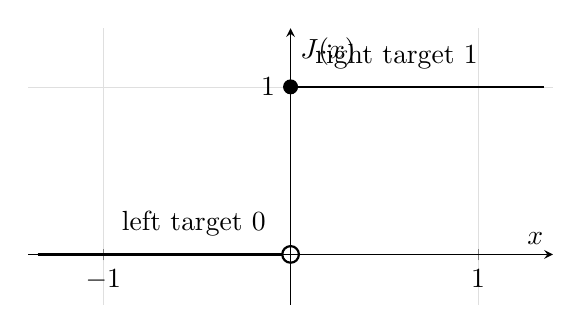
\begin{tikzpicture}
\begin{axis}[
    width=0.68\textwidth,
    height=0.42\textwidth,
    xmin=-1.4, xmax=1.4,
    ymin=-0.3, ymax=1.35,
    axis lines=middle,
    xlabel={\(x\)},
    ylabel={\(J(x)\)},
    xtick={-1,0,1},
    ytick={0,1},
    grid=both,
    grid style={line width=.1pt, draw=gray!25},
]
\addplot[thick, domain=-1.35:-0.04, samples=2] {0};
\addplot[thick, domain=0:1.35, samples=2] {1};
\addplot[only marks, mark=o, mark size=3pt, thick] coordinates {(0,0)};
\addplot[only marks, mark=*, mark size=2.5pt] coordinates {(0,1)};
\node[anchor=south east] at (axis cs:-0.08,0.05) {left target \(0\)};
\node[anchor=south west] at (axis cs:0.08,1.05) {right target \(1\)};
\end{axis}
\end{tikzpicture}
\caption{A jump creates two different one-sided limits, so the two-sided limit fails.}
\label{fig:jump-warning-no-limit}
\end{figure}

Changing the value at \(x=0\) cannot repair the two-sided limit.  The problem is not the point itself.  The problem is that the nearby values on the two sides head toward different numbers.

\[
\boxed{\text{A two-sided limit is about agreement from both sides.}}
\]

\subsection{A limit that is infinite, not finite}
\label{subsec:infinite-not-finite-warning}

A different kind of failure happens when the values do not settle near any finite number.

Consider

\[
f(x)=\frac{1}{x^2},
\qquad x\neq0.
\]

As \(x\) gets close to \(0\), the denominator \(x^2\) gets close to \(0\), but stays positive.  The quotient grows larger and larger.

\[
\begin{array}{c|cccccc}
x & -0.1 & -0.01 & -0.001 & 0.001 & 0.01 & 0.1 \\ \hline
\dfrac1{x^2} & 100 & 10{,}000 & 1{,}000{,}000
& 1{,}000{,}000 & 10{,}000 & 100
\end{array}
\]

We write

\[
\lim_{x\to0}\frac1{x^2}=\infty.
\]

This notation does not mean that the function has a finite limit.  It means the values grow beyond every fixed positive bound.

There is no real number \(L\) such that

\[
\lim_{x\to0}\frac1{x^2}=L.
\]

\begin{figure}[h]
\centering
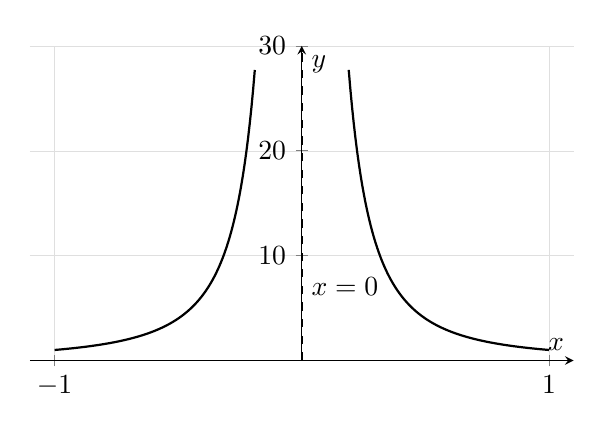
\begin{tikzpicture}
\begin{axis}[
    width=0.70\textwidth,
    height=0.46\textwidth,
    xmin=-1.1, xmax=1.1,
    ymin=0, ymax=30,
    axis lines=middle,
    xlabel={\(x\)},
    ylabel={\(y\)},
    xtick={-1,0,1},
    ytick={10,20,30},
    grid=both,
    grid style={line width=.1pt, draw=gray!25},
]
\addplot[thick, domain=-1:-0.19, samples=120] {1/(x^2)};
\addplot[thick, domain=0.19:1, samples=120] {1/(x^2)};
\draw[dashed, thick] (axis cs:0,0) -- (axis cs:0,30);
\node[anchor=west] at (axis cs:0.0,7) {\(x=0\)};
\end{axis}
\end{tikzpicture}
\caption{The values of \(1/x^2\) grow without bound near \(0\).  This is infinite behavior, not a finite limit.}
\label{fig:infinite-limit-warning}
\end{figure}

A removable discontinuity can be repaired by filling in one value.  Infinite divergent behavior cannot.  No choice of \(f(0)\) can keep the nearby values close to a finite number.

\[
\boxed{\infty\text{ describes unbounded behavior.  It is not a real-number target.}}
\]

\subsection{The Intermediate Value Theorem fails without continuity}
\label{subsec:ivt-fails-without-continuity-warning}

The Intermediate Value Theorem said:

\[
\text{continuous graph}+\text{endpoint values}
\quad\Longrightarrow\quad
\text{all intermediate values are hit.}
\]

The word \emph{continuous} cannot be removed.

Define

\[
S(x)=
\begin{cases}
0, & x<0,\\
2, & x\ge0.
\end{cases}
\]

On the interval \([-1,1]\),

\[
S(-1)=0
\qquad\text{and}\qquad
S(1)=2.
\]

The number \(1\) lies between \(0\) and \(2\).  If we tried to use the Intermediate Value Theorem, we might expect some \(c\in[-1,1]\) such that

\[
S(c)=1.
\]

But no such \(c\) exists.  The function takes only the values \(0\) and \(2\).  It jumps over \(1\).

\begin{figure}[h]
\centering
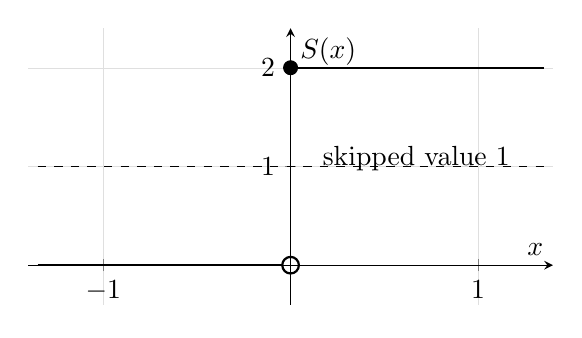
\begin{tikzpicture}
\begin{axis}[
    width=0.68\textwidth,
    height=0.42\textwidth,
    xmin=-1.4, xmax=1.4,
    ymin=-0.4, ymax=2.4,
    axis lines=middle,
    xlabel={\(x\)},
    ylabel={\(S(x)\)},
    xtick={-1,0,1},
    ytick={0,1,2},
    grid=both,
    grid style={line width=.1pt, draw=gray!25},
]
\addplot[thick, domain=-1.35:-0.04, samples=2] {0};
\addplot[thick, domain=0:1.35, samples=2] {2};
\addplot[only marks, mark=o, mark size=3pt, thick] coordinates {(0,0)};
\addplot[only marks, mark=*, mark size=2.5pt] coordinates {(0,2)};
\draw[dashed] (axis cs:-1.35,1) -- (axis cs:1.35,1);
\node[anchor=west] at (axis cs:0.12,1.08) {skipped value \(1\)};
\end{axis}
\end{tikzpicture}
\caption{Without continuity, a function can jump over an intermediate value.}
\label{fig:ivt-warning-fails}
\end{figure}

The theorem fails because \(S\) is not continuous at \(0\).

\[
\boxed{\text{The Intermediate Value Theorem is a no-jump theorem.}}
\]

\subsection{The Extreme Value Theorem fails on an open interval}
\label{subsec:evt-fails-open-interval-warning}

The Extreme Value Theorem said:

\[
\text{continuous on }[a,b]
\quad\Longrightarrow\quad
\text{absolute maximum and minimum are reached.}
\]

The closed interval \([a,b]\) includes its endpoints.  If the endpoints are missing, the conclusion can fail.

Consider

\[
f(x)=x
\]

on the open interval

\[
(0,1).
\]

The function is continuous at every point of its domain.  Its values get close to \(1\), but never equal \(1\), because \(x=1\) is not in the interval.

So \(f\) has no absolute maximum on \((0,1)\).

The values also get close to \(0\), but never equal \(0\), because \(x=0\) is not in the interval.

So \(f\) has no absolute minimum on \((0,1)\).

\begin{figure}[h]
\centering
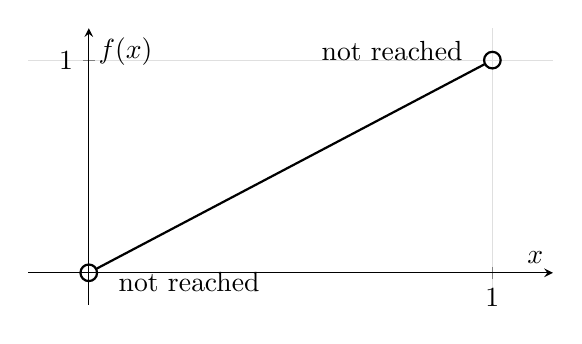
\begin{tikzpicture}
\begin{axis}[
    width=0.68\textwidth,
    height=0.42\textwidth,
    xmin=-0.15, xmax=1.15,
    ymin=-0.15, ymax=1.15,
    axis lines=middle,
    xlabel={\(x\)},
    ylabel={\(f(x)\)},
    xtick={0,1},
    ytick={0,1},
    grid=both,
    grid style={line width=.1pt, draw=gray!25},
]
\addplot[thick, domain=0.02:0.98, samples=2] {x};
\addplot[only marks, mark=o, mark size=3pt, thick] coordinates {(0,0) (1,1)};
\node[anchor=south east] at (axis cs:0.95,0.95) {not reached};
\node[anchor=north west] at (axis cs:0.05,0.05) {not reached};
\end{axis}
\end{tikzpicture}
\caption{On \((0,1)\), the function \(f(x)=x\) approaches its lowest and highest possible values but never reaches them.}
\label{fig:evt-warning-open-interval}
\end{figure}

The problem is not the formula.  The formula \(f(x)=x\) is perfectly continuous.  The problem is the domain.  The endpoints are missing.

\[
\boxed{\text{For the Extreme Value Theorem, endpoints matter.}}
\]

\subsection{The Extreme Value Theorem fails on an unbounded interval}
\label{subsec:evt-fails-unbounded-interval-warning}

A closed interval is not enough if it stretches forever.

Consider

\[
f(x)=x
\]

on

\[
[0,\infty).
\]

The function is continuous on its domain.  The interval includes its left endpoint \(0\), so \(f\) has an absolute minimum:

\[
f(0)=0.
\]

But \(f\) has no absolute maximum.  Given any value \(f(x)=x\), we can choose a larger input, such as \(x+1\), and get

\[
f(x+1)=x+1>f(x).
\]

So no largest value exists.

A physical version is also common.  Recall the cooling model

\[
T(t)=70+\frac{90}{t+1},
\qquad t\ge0.
\]

The interval \([0,\infty)\) is unbounded.  The temperature starts at

\[
T(0)=160,
\]

and approaches \(70\) as \(t\to\infty\).  It never reaches \(70\) for any finite \(t\), because

\[
\frac{90}{t+1}>0.
\]

So this continuous function has an absolute maximum on \([0,\infty)\), but no absolute minimum.

\[
\boxed{\text{A function can approach a best value forever without reaching it.}}
\]

The word ``bounded'' in the Extreme Value Theorem prevents this escape to infinity.

\subsection{A map of the warnings}
\label{subsec:map-of-warnings}

The examples above are not exceptions to the theorems.  They are reminders of what the theorems actually say.

\begin{center}
\begin{tabular}{c|c|c}
\textbf{claim we want} & \textbf{missing hypothesis} & \textbf{what breaks} \\ \hline
\(\lim_{x\to a}f(x)\) exists &
left and right sides agree &
jump gives two targets \\[3pt]
finite limit exists &
values stay bounded near \(a\) &
vertical asymptote \\[3pt]
IVT conclusion &
continuity &
intermediate value can be skipped \\[3pt]
EVT conclusion &
closed interval &
endpoint value may not be reached \\[3pt]
EVT conclusion &
bounded interval &
largest or smallest value may escape to infinity
\end{tabular}
\end{center}

A theorem is a machine with conditions.  If a condition is missing, the output is no longer guaranteed.

Limits and continuity have now given us a careful language for functions of a real variable \(x\).  But some limiting processes arrive as lists:

\[
1,\quad \frac12,\quad \frac13,\quad \frac14,\quad \ldots
\]

or

\[
1.4,\quad 1.41,\quad 1.414,\quad 1.4142,\quad \ldots
\]

The input is no longer every nearby real number.  The input is the whole-number step \(n\).  That leads to sequences.

\section{Sequences as limits indexed by whole numbers}
\label{sec:sequences-as-limits-indexed}

Limits so far have used a real input approaching a point:

\[
x\to a,
\qquad
x\to\infty.
\]

But many approximations arrive one step at a time.  Bisection gives a first interval, then a second, then a third.  A decimal approximation gives a first decimal, then a second, then a third.

The input is not a continuous variable.  It is a counting number:

\[
n=1,2,3,\ldots
\]

A limit of such a list is called a limit of a sequence.

\subsection{Sequence notation}
\label{subsec:sequence-notation}

A \emph{sequence} is a function whose input is a positive integer.

Instead of writing

\[
a(1),\quad a(2),\quad a(3),\ldots,
\]

we usually write

\[
a_1,\quad a_2,\quad a_3,\ldots.
\]

The number \(a_n\) is called the \(n\)th term of the sequence.

\paragraph{Example.}
The formula

\[
a_n=\frac1n
\]

gives the sequence

\[
1,\quad \frac12,\quad \frac13,\quad \frac14,\quad \frac15,\quad \ldots.
\]

Here

\[
a_1=1,
\qquad
a_2=\frac12,
\qquad
a_{10}=\frac1{10}.
\]

\paragraph{Example.}
The formula

\[
b_n=(-1)^n
\]

gives

\[
-1,\quad 1,\quad -1,\quad 1,\quad \ldots.
\]

This sequence does not settle down.  It alternates forever.

\paragraph{Example: recursive notation.}
Some sequences are not first given by an explicit formula.  They are given by a starting value and a rule for the next term.

Let

\[
x_1=1,
\]

and

\[
x_{n+1}=\frac{x_n+2}{2}.
\]

Then

\[
x_2=\frac{1+2}{2}=\frac32,
\]

\[
x_3=\frac{\frac32+2}{2}=\frac74,
\]

\[
x_4=\frac{\frac74+2}{2}=\frac{15}{8}.
\]

So the sequence begins

\[
1,\quad \frac32,\quad \frac74,\quad \frac{15}{8},\quad \ldots.
\]

The terms move toward \(2\).  Each step takes the current value and moves halfway from it to \(2\).

Recursive sequences will appear later in Newton's method and Euler's method.  They are how a computer often follows a mathematical process step by step.

\subsection{Convergence and divergence}
\label{subsec:sequence-convergence-divergence}

The sequence

\[
a_n=\frac1n
\]

approaches \(0\).  The terms are positive, but they can be made as close to \(0\) as we want by taking \(n\) large enough.

We write

\[
\lim_{n\to\infty}\frac1n=0.
\]

The notation \(n\to\infty\) means that the index \(n\) grows without bound.

\begin{quote}
\textbf{Limit of a sequence, informally.}
We write

\[
\lim_{n\to\infty}a_n=L
\]

if the terms \(a_n\) approach the number \(L\) as \(n\) becomes arbitrarily large.
\end{quote}

A sequence that has a finite limit is called \emph{convergent}.  A sequence that does not have a finite limit is called \emph{divergent}.

The precise definition is the same epsilon idea we used for functions, with \(\delta\) replaced by a cutoff index \(N\).

\begin{quote}
\textbf{Precise definition of sequence convergence.}
We write

\[
\lim_{n\to\infty}a_n=L
\]

if for every \(\varepsilon>0\), there exists a positive integer \(N\) such that whenever

\[
n\ge N,
\]

we have

\[
|a_n-L|<\varepsilon.
\]
\end{quote}

The order matters again.

\[
\boxed{
\text{First comes the allowed error }\varepsilon.
\quad
\text{Then we choose a cutoff }N.
}
\]

After that cutoff, every term must stay inside the \(\varepsilon\)-window around \(L\).

\paragraph{Example: proving \(1/n\to0\).}
We prove that

\[
\lim_{n\to\infty}\frac1n=0.
\]

Let \(\varepsilon>0\) be given.  Choose a positive integer \(N\) such that

\[
N>\frac1{\varepsilon}.
\]

If \(n\ge N\), then

\[
n>\frac1{\varepsilon},
\]

so

\[
\frac1n<\varepsilon.
\]

Therefore

\[
\left|\frac1n-0\right|<\varepsilon.
\]

Thus

\[
\lim_{n\to\infty}\frac1n=0.
\]

\paragraph{Example: a rational expression.}
Find

\[
\lim_{n\to\infty}\frac{2n+1}{n+3}.
\]

Divide numerator and denominator by \(n\):

\[
\frac{2n+1}{n+3}
=
\frac{2+\frac1n}{1+\frac3n}.
\]

As \(n\to\infty\),

\[
\frac1n\to0
\qquad\text{and}\qquad
\frac3n\to0.
\]

So

\[
\lim_{n\to\infty}\frac{2n+1}{n+3}
=
\frac{2+0}{1+0}
=
2.
\]

We can also see the error directly:

\[
\left|\frac{2n+1}{n+3}-2\right|
=
\left|\frac{2n+1-2n-6}{n+3}\right|
=
\frac5{n+3}.
\]

This error approaches \(0\).

\begin{figure}[h]
\centering
\begin{minipage}{0.47\textwidth}
\centering
\begin{tikzpicture}
\begin{axis}[
    width=\textwidth,
    height=0.70\textwidth,
    xmin=0.5, xmax=8.5,
    ymin=-0.05, ymax=1.1,
    axis lines=left,
    xlabel={\(n\)},
    ylabel={\(a_n\)},
    xtick={1,2,3,4,5,6,7,8},
    ytick={0,0.5,1},
    title={\(\displaystyle a_n=\frac1n\)},
    grid=both,
    grid style={line width=.1pt, draw=gray!25},
]
\addplot[only marks, mark=*] coordinates {
(1,1) (2,0.5) (3,0.3333) (4,0.25) (5,0.2) (6,0.1667) (7,0.1429) (8,0.125)
};
\addplot[dashed, domain=0.5:8.5, samples=2] {0};
\end{axis}
\end{tikzpicture}
\end{minipage}
\hfill
\begin{minipage}{0.47\textwidth}
\centering
\begin{tikzpicture}
\begin{axis}[
    width=\textwidth,
    height=0.70\textwidth,
    xmin=0.5, xmax=8.5,
    ymin=-1.3, ymax=1.3,
    axis lines=left,
    xlabel={\(n\)},
    ylabel={\(b_n\)},
    xtick={1,2,3,4,5,6,7,8},
    ytick={-1,0,1},
    title={\(\displaystyle b_n=(-1)^n\)},
    grid=both,
    grid style={line width=.1pt, draw=gray!25},
]
\addplot[only marks, mark=*] coordinates {
(1,-1) (2,1) (3,-1) (4,1) (5,-1) (6,1) (7,-1) (8,1)
};
\addplot[dashed, domain=0.5:8.5, samples=2] {1};
\addplot[dashed, domain=0.5:8.5, samples=2] {-1};
\end{axis}
\end{tikzpicture}
\end{minipage}
\caption{The sequence \(1/n\) settles toward \(0\).  The sequence \((-1)^n\) keeps jumping between two values.}
\label{fig:sequence-convergent-divergent}
\end{figure}

\paragraph{Example: an oscillating sequence.}
The sequence

\[
b_n=(-1)^n
\]

diverges.

The even terms are

\[
b_2=b_4=b_6=\cdots=1.
\]

The odd terms are

\[
b_1=b_3=b_5=\cdots=-1.
\]

The terms cannot approach one number.  They keep returning to \(1\) and \(-1\).

This is the sequence version of a jump limit.  A limit needs one target.

\paragraph{Example: growing without bound.}
The sequence

\[
c_n=n
\]

also diverges.  It does not oscillate.  It grows without bound:

\[
1,\quad 2,\quad 3,\quad 4,\quad \ldots.
\]

We write

\[
\lim_{n\to\infty}n=\infty
\]

to describe this growth, but this is not convergence to a real number.

\[
\boxed{\text{Convergent means approaching a finite real number.}}
\]

\subsection{Monotone bounded sequences}
\label{subsec:monotone-bounded-sequences}

Some sequences converge because they move steadily in one direction and cannot escape.

The decimal approximations

\[
1.4,\quad 1.41,\quad 1.414,\quad 1.4142,\quad \ldots
\]

move upward toward \(\sqrt2\).  They never pass \(\sqrt2\).  They are increasing and bounded above.

This is a common pattern.

\begin{quote}
\textbf{Monotone sequences.}
A sequence \((a_n)\) is \emph{increasing} if

\[
a_{n+1}\ge a_n
\]

for every \(n\).

It is \emph{decreasing} if

\[
a_{n+1}\le a_n
\]

for every \(n\).

A sequence is \emph{monotone} if it is increasing or decreasing.
\end{quote}

Here ``increasing'' allows equality.  Some books call this \emph{nondecreasing}.

\begin{quote}
\textbf{Bounded sequences.}
A sequence \((a_n)\) is \emph{bounded above} if there is a number \(B\) such that

\[
a_n\le B
\]

for every \(n\).

It is \emph{bounded below} if there is a number \(A\) such that

\[
A\le a_n
\]

for every \(n\).

It is \emph{bounded} if it is bounded above and bounded below.
\end{quote}

\paragraph{Example.}
Let

\[
a_n=1-\frac1n.
\]

The sequence begins

\[
0,\quad \frac12,\quad \frac23,\quad \frac34,\quad \frac45,\quad \ldots.
\]

It is increasing.  Indeed,

\[
a_{n+1}-a_n
=
\left(1-\frac1{n+1}\right)-\left(1-\frac1n\right)
=
\frac1n-\frac1{n+1}
=
\frac1{n(n+1)}
>
0.
\]

It is bounded above by \(1\), since

\[
1-\frac1n<1.
\]

The sequence converges to \(1\):

\[
\lim_{n\to\infty}\left(1-\frac1n\right)=1.
\]

\begin{figure}[h]
\centering
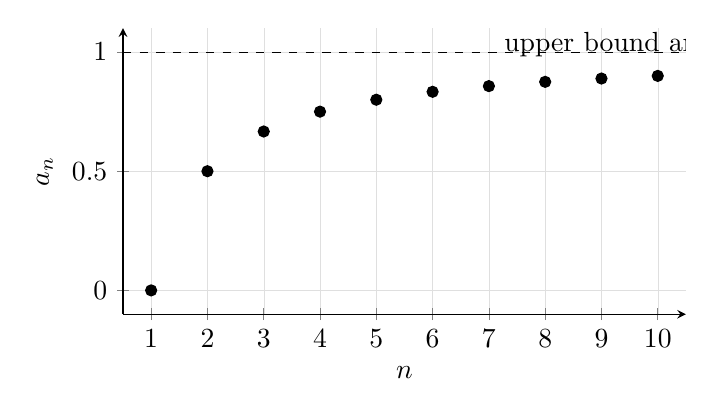
\begin{tikzpicture}
\begin{axis}[
    width=0.72\textwidth,
    height=0.43\textwidth,
    xmin=0.5, xmax=10.5,
    ymin=-0.1, ymax=1.1,
    axis lines=left,
    xlabel={\(n\)},
    ylabel={\(a_n\)},
    xtick={1,2,3,4,5,6,7,8,9,10},
    ytick={0,0.5,1},
    grid=both,
    grid style={line width=.1pt, draw=gray!25},
]
\addplot[only marks, mark=*] coordinates {
(1,0) (2,0.5) (3,0.6667) (4,0.75) (5,0.8)
(6,0.8333) (7,0.8571) (8,0.875) (9,0.8889) (10,0.9)
};
\addplot[dashed, domain=0.5:10.5, samples=2] {1};
\node[anchor=west] at (axis cs:7.1,1.03) {upper bound and limit \(1\)};
\end{axis}
\end{tikzpicture}
\caption{The sequence \(a_n=1-1/n\) increases toward \(1\) without passing it.}
\label{fig:monotone-bounded-sequence}
\end{figure}

The theorem behind this example is one of the first places where the completeness of the real numbers matters.

\begin{quote}
\textbf{Monotone Bounded Sequence Theorem.}
Every increasing sequence that is bounded above converges.

Every decreasing sequence that is bounded below converges.
\end{quote}

\paragraph{Proof for the increasing case.}
Let \((a_n)\) be increasing and bounded above.  Consider the set of its terms:

\[
\{a_1,a_2,a_3,\ldots\}.
\]

Since the sequence is bounded above, this set has an upper bound.  By the least upper bound property, it has a least upper bound.  Call it \(L\).

We claim that

\[
a_n\to L.
\]

Let \(\varepsilon>0\) be given.  Since \(L\) is the least upper bound, the number

\[
L-\varepsilon
\]

is not an upper bound.  Therefore at least one term of the sequence lies above it.  That is, there is an integer \(N\) such that

\[
a_N>L-\varepsilon.
\]

Because the sequence is increasing, for every \(n\ge N\),

\[
a_n\ge a_N.
\]

Also, since \(L\) is an upper bound,

\[
a_n\le L.
\]

Thus, for every \(n\ge N\),

\[
L-\varepsilon<a_n\le L.
\]

So

\[
|a_n-L|<\varepsilon.
\]

Therefore

\[
a_n\to L.
\]

The decreasing case is similar, or can be proved by applying the increasing case to \(-a_n\).

\paragraph{Why the hypotheses matter.}
Increasing alone is not enough.  The sequence

\[
a_n=n
\]

is increasing, but it is not bounded above.  It diverges to infinity.

Bounded alone is not enough.  The sequence

\[
b_n=(-1)^n
\]

is bounded, because

\[
-1\le b_n\le1
\]

for every \(n\).  But it is not monotone, and it diverges.

\[
\boxed{
\text{Monotone controls direction.}
\qquad
\text{Bounded prevents divergence to infinity.}
}
\]

Together, they force convergence.

\subsection{Bisection as a sequence}
\label{subsec:bisection-as-sequence}

The bisection method from the Intermediate Value Theorem produces sequences automatically.

For

\[
p(x)=x^3-x-1,
\]

we found a root in \([1,2]\).  Bisection creates nested intervals

\[
[L_1,R_1]\supset [L_2,R_2]\supset [L_3,R_3]\supset\cdots
\]

where each interval still contains a sign change.

The left endpoints form an increasing sequence:

\[
L_1\le L_2\le L_3\le\cdots.
\]

The right endpoints form a decreasing sequence:

\[
R_1\ge R_2\ge R_3\ge\cdots.
\]

The left endpoints are bounded above by \(2\).  The right endpoints are bounded below by \(1\).  Therefore both endpoint sequences converge.

Also, the interval lengths shrink by a factor of \(\frac12\) at each step.  If the first interval has length \(1\), then after \(n\) steps the length is

\[
\frac1{2^n}.
\]

Since

\[
\frac1{2^n}\to0,
\]

the two endpoint sequences converge to the same number.  That number is the root trapped by bisection.

This is why bisection is reliable.  It does not guess wildly.  It creates sequences that are forced to settle.

\subsection{Sequences as preparation for infinite series}
\label{subsec:sequences-prepare-series}

A sequence is one infinite list of numbers.  An infinite series is an infinite sum.

But an infinite sum is understood through a sequence.

Consider

\[
\frac12+\frac14+\frac18+\frac1{16}+\cdots.
\]

We do not add infinitely many terms all at once.  We add the first \(N\) terms and watch what happens as \(N\to\infty\).

Define the partial sums

\[
s_N=\frac12+\frac14+\frac18+\cdots+\frac1{2^N}.
\]

Then

\[
s_1=\frac12,
\]

\[
s_2=\frac12+\frac14=\frac34,
\]

\[
s_3=\frac12+\frac14+\frac18=\frac78.
\]

In general,

\[
s_N=1-\frac1{2^N}.
\]

Since

\[
\frac1{2^N}\to0,
\]

we get

\[
s_N\to1.
\]

So we write

\[
\frac12+\frac14+\frac18+\frac1{16}+\cdots=1.
\]

More compactly,

\[
\sum_{n=1}^{\infty}\frac1{2^n}=1.
\]

The infinite series converges because its sequence of partial sums converges.

\begin{quote}
\textbf{Series as a sequence problem.}
An infinite series

\[
\sum_{n=1}^{\infty}a_n
\]

converges if the sequence of partial sums

\[
s_N=a_1+a_2+\cdots+a_N
\]

converges.
\end{quote}

This distinction matters.  The terms of a series and the partial sums of a series are different sequences.

For example,

\[
\frac1n\to0.
\]

That means the individual terms of

\[
\sum_{n=1}^{\infty}\frac1n
\]

get small.  But it does not yet say that the accumulated sum settles down.  Later we will see that

\[
\sum_{n=1}^{\infty}\frac1n
\]

diverges, even though its terms approach \(0\).

\[
\boxed{
\text{Small terms are necessary for a series to converge, but not sufficient.}
}
\]

Sequences are the bridge from limits to infinite sums.  They also bring us back to the question that started the chapter.  A tangent slope can be approached by a sequence of secant slopes, for example by taking

\[
h=\frac1n.
\]

Then

\[
\frac{f(a+\frac1n)-f(a)}{\frac1n}
\]

is a sequence.  If those slopes settle toward one number, the graph is telling us its instantaneous rate of change.

That number will be the derivative.
\section{Chapter review and discovery problems}
\label{sec:chapter3-review-discovery}

This chapter began with one small calculation:

\[
\frac{(2+h)^2-2^2}{h}=4+h,
\qquad h\neq0.
\]

The forbidden value \(h=0\) did not stop us from seeing what happens as \(h\) gets close to \(0\).  That idea became the language of limits.  Limits then gave us continuity, one-sided behavior, infinite behavior, asymptotes, sequences, and two existence theorems.

Before we use limits to define derivatives, it is worth pausing to see the whole map.

\subsection{The chapter in one picture}
\label{subsec:chapter3-one-picture}

A limit is the central idea.  The other ideas in the chapter are different ways of asking what a limit is doing.

\begin{figure}[h]
\centering
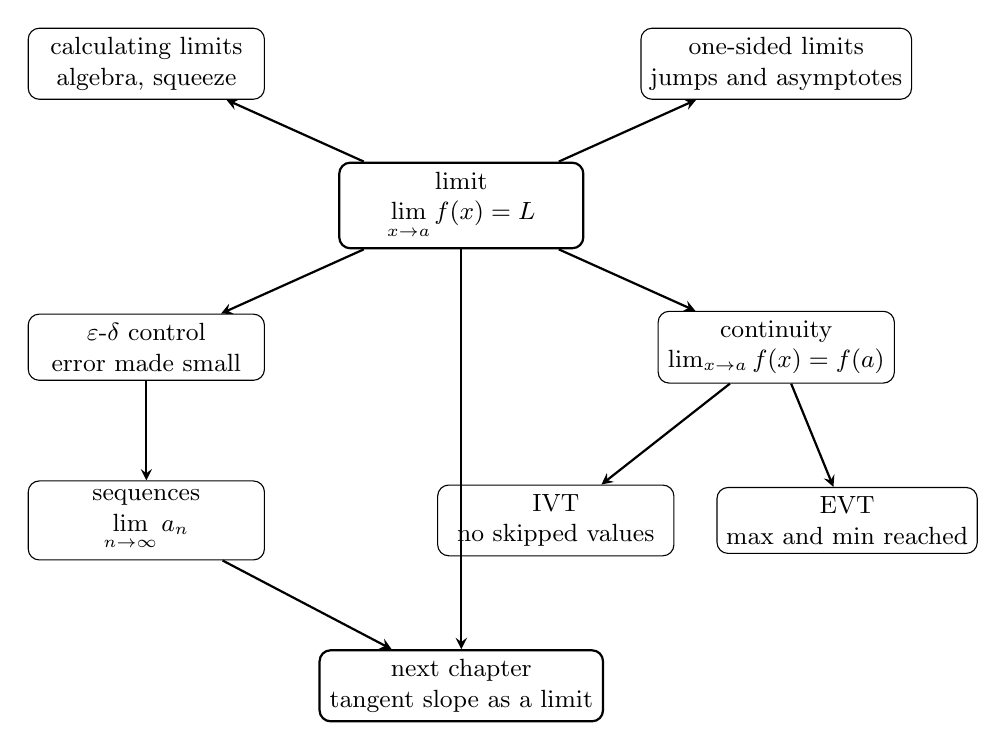
\begin{tikzpicture}[every node/.style={font=\small}, >=stealth]
  \node[draw, rounded corners, thick, align=center, minimum width=3.1cm, minimum height=0.9cm] (limit) at (0,0)
    {limit\\ \(\displaystyle \lim_{x\to a}f(x)=L\)};

  \node[draw, rounded corners, align=center, minimum width=3.0cm] (calc) at (-4,1.8)
    {calculating limits\\ algebra, squeeze};
  \node[draw, rounded corners, align=center, minimum width=3.0cm] (oneside) at (4,1.8)
    {one-sided limits\\ jumps and asymptotes};
  \node[draw, rounded corners, align=center, minimum width=3.0cm] (precise) at (-4,-1.8)
    {\(\varepsilon\)-\(\delta\) control\\ error made small};
  \node[draw, rounded corners, align=center, minimum width=3.0cm] (cont) at (4,-1.8)
    {continuity\\ \(\lim_{x\to a}f(x)=f(a)\)};

  \node[draw, rounded corners, align=center, minimum width=3.0cm] (ivt) at (1.2,-4.0)
    {IVT\\ no skipped values};
  \node[draw, rounded corners, align=center, minimum width=3.0cm] (evt) at (4.9,-4.0)
    {EVT\\ max and min reached};
  \node[draw, rounded corners, align=center, minimum width=3.0cm] (seq) at (-4,-4.0)
    {sequences\\ \(\displaystyle \lim_{n\to\infty}a_n\)};

  \node[draw, rounded corners, thick, align=center, minimum width=3.6cm, minimum height=0.9cm] (deriv) at (0,-6.1)
    {next chapter\\ tangent slope as a limit};

  \draw[->, thick] (limit) -- (calc);
  \draw[->, thick] (limit) -- (oneside);
  \draw[->, thick] (limit) -- (precise);
  \draw[->, thick] (limit) -- (cont);
  \draw[->, thick] (cont) -- (ivt);
  \draw[->, thick] (cont) -- (evt);
  \draw[->, thick] (precise) -- (seq);
  \draw[->, thick] (seq) -- (deriv);
  \draw[->, thick] (limit) -- (deriv);
\end{tikzpicture}
\caption{Limits are the center.  Continuity, asymptotes, sequences, and tangent slopes all use the same idea of controlled approach.}
\label{fig:chapter3-concept-map}
\end{figure}

The most important habit is not memorizing a table of limit forms.  It is asking:

\[
\text{What is the input doing, and what target is the output approaching?}
\]

\subsection{A decision guide for limits and continuity}
\label{subsec:chapter3-decision-guide}

When you face a limit problem, begin with the simplest test.  Then move only as far as the problem requires.

\[
\begin{array}{>{\centering\arraybackslash}p{0.35\textwidth}|p{0.58\textwidth}}
\textbf{what you see} & \textbf{what to try} \\ \hline
direct substitution gives a real number &
Use continuity or the limit laws. \\[4pt]
direct substitution gives \(\dfrac00\) &
Factor, cancel, expand, combine fractions, or rationalize.  Then try again. \\[8pt]
left and right sides behave differently &
Compute one-sided limits.  A two-sided limit exists only if they agree. \\[6pt]
denominator approaches \(0\) without cancellation &
Check signs from the left and right.  The limit may be \(\infty\), \(-\infty\), or may fail to exist. \\[6pt]
\(x\to\infty\) or \(x\to-\infty\) &
Divide by the largest power, or compare leading terms. \\[6pt]
an oscillating factor is multiplied by something small &
Try the squeeze principle. \\[6pt]
a theorem about continuous functions is tempting &
Check the hypotheses first: continuity, closed interval, bounded interval, and the right endpoint information. \\[6pt]
a sequence appears &
Use the \(\varepsilon\)-\(N\) definition, algebraic limit laws, or monotone bounded convergence.
\end{array}
\]

The warning examples in Section \ref{sec:warning-examples-limits-continuity} should stay close by.  Most mistakes come from using a true theorem without checking the conditions that make it true.

\subsection{Review problems}
\label{subsec:chapter3-review-problems}

The problems below are grouped by purpose.  Some are computational.  Some ask for explanations.  Some ask for proof.  In the proof problems, the goal is not speed.  The goal is control.

\subsubsection*{A. Concept checks}

\begin{enumerate}
\item Explain the difference between

\[
\lim_{x\to a}f(x)
\qquad\text{and}\qquad
f(a).
\]

Give an example where the limit exists but does not equal the function value.

\item Explain why the condition

\[
0<|x-a|<\delta
\]

appears in the definition of a limit.

\item What does the statement

\[
\lim_{x\to a}f(x)=\infty
\]

mean?  Why is this not convergence to a real number?

\item A table gives values of \(f(x)\) near \(x=3\), and the values appear to approach \(8\).  Why is the table useful?  Why is it not, by itself, a proof?

\item State the two-sided limit test using left-hand and right-hand limits.

\item In your own words, explain what continuity at \(a\) means.

\item Why can a removable discontinuity be repaired by changing one value, but a jump discontinuity cannot?

\item State the Intermediate Value Theorem.  Name its main hypothesis.

\item State the Extreme Value Theorem.  Explain why both words ``closed'' and ``bounded'' matter in the interval hypothesis.

\item Explain the difference between convergence of a sequence and convergence of a series.  Use the words \emph{terms} and \emph{partial sums}.
\end{enumerate}

\subsubsection*{B. Skills: compute and interpret limits}

Compute each limit if it exists as a finite real number.  If no finite two-sided limit exists, explain why.  When appropriate, give one-sided limits.

\begin{enumerate}
\item Polynomial and rational limits.

\[
\lim_{x\to4}(3x^2-5x+1),
\qquad
\lim_{x\to-2}\frac{x^2+1}{x-3},
\]

\[
\lim_{x\to0}\frac{5x^3-2x+7}{x^2+1},
\qquad
\lim_{x\to3}\frac{x^2-9}{x+1}.
\]

\item Removable discontinuities.

\[
\lim_{x\to3}\frac{x^2-9}{x-3},
\qquad
\lim_{x\to2}\frac{x^3-8}{x-2},
\]

\[
\lim_{x\to4}\frac{\sqrt{x+5}-3}{x-4},
\qquad
\lim_{x\to2}\frac{\frac1x-\frac12}{x-2}.
\]

\item Squeeze principle.

\[
\lim_{x\to0}x\sin\frac1x,
\qquad
\lim_{x\to0}x^2\cos\frac1{x^2},
\]

\[
\lim_{x\to0}|x|\sin\frac1x.
\]

For each one, write the inequalities that trap the function.

\item One-sided limits for a piecewise function.  Let

\[
F(x)=
\begin{cases}
x^2+2, & x<1,\\
4, & x=1,\\
3x, & x>1.
\end{cases}
\]

Find

\[
\lim_{x\to1^-}F(x),
\qquad
\lim_{x\to1^+}F(x),
\qquad
\lim_{x\to1}F(x),
\qquad
F(1).
\]

Is \(F\) continuous at \(1\)?

\item Another piecewise function.  Let

\[
G(x)=
\begin{cases}
2x+1, & x<2,\\
5, & x=2,\\
x^2-1, & x>2.
\end{cases}
\]

Find the left-hand limit, right-hand limit, two-sided limit, and function value at \(x=2\).  Is this a removable discontinuity, a jump discontinuity, or neither?

\item Infinite limits.

\[
\lim_{x\to3^-}\frac1{x-3},
\qquad
\lim_{x\to3^+}\frac1{x-3},
\]

\[
\lim_{x\to3}\frac1{(x-3)^2},
\qquad
\lim_{x\to2^-}\frac{x+2}{x^2-4},
\qquad
\lim_{x\to2^+}\frac{x+2}{x^2-4}.
\]

For each function, identify any vertical asymptote.

\item Limits at infinity.

\[
\lim_{x\to\infty}\frac{5x^2-x+1}{2x^2+3},
\qquad
\lim_{x\to-\infty}\frac{5x^2-x+1}{2x^2+3},
\]

\[
\lim_{x\to\infty}\frac{3x+7}{x^2+1},
\qquad
\lim_{x\to\infty}\frac{x^2+1}{x-1}.
\]

For the last function, decide whether there is a horizontal asymptote or a slant asymptote.

\item Slant asymptote.  Write

\[
\frac{x^2+3x}{x+1}
\]

in the form

\[
mx+b+\frac{r}{x+1}.
\]

Then find the slant asymptote as \(x\to\infty\) and as \(x\to-\infty\).

\item Sequence limits.

\[
\lim_{n\to\infty}\frac{3n+1}{2n-5},
\qquad
\lim_{n\to\infty}\left(1-\frac1n\right),
\]

\[
\lim_{n\to\infty}\frac{n^2+4}{5n^2-n},
\qquad
\lim_{n\to\infty}(-1)^n.
\]

Classify each sequence as convergent or divergent.

\item Monotone bounded sequences.  For each sequence, decide whether it is increasing, decreasing, bounded above, bounded below, and convergent.

\[
a_n=1-\frac1n,
\qquad
b_n=\frac1n,
\qquad
c_n=n,
\qquad
d_n=(-1)^n.
\]
\end{enumerate}

\subsubsection*{C. Reading limits from a graph}

Use Figure \ref{fig:chapter3-graph-reading-review} for the next problem.

\begin{figure}[h]
\centering
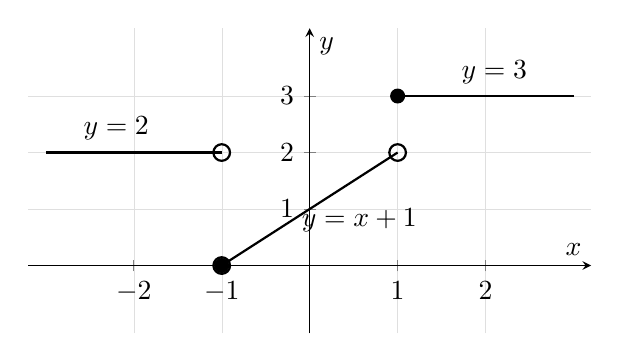
\begin{tikzpicture}
\begin{axis}[
    width=0.72\textwidth,
    height=0.45\textwidth,
    xmin=-3.2, xmax=3.2,
    ymin=-1.2, ymax=4.2,
    axis lines=middle,
    xlabel={\(x\)},
    ylabel={\(y\)},
    xtick={-2,-1,0,1,2},
    ytick={0,1,2,3},
    grid=both,
    grid style={line width=.1pt, draw=gray!25},
]
\addplot[thick, domain=-3:-1, samples=2] {2};
\addplot[thick, domain=-1:1, samples=2] {x+1};
\addplot[thick, domain=1:3, samples=2] {3};
\addplot[only marks, mark=o, mark size=3pt, thick] coordinates {(-1,2) (-1,0) (1,2)};
\addplot[only marks, mark=*, mark size=2.5pt] coordinates {(-1,0) (1,3)};
\node[anchor=south] at (axis cs:-2.2,2.05) {\(y=2\)};
\node[anchor=west] at (axis cs:-0.2,0.8) {\(y=x+1\)};
\node[anchor=south] at (axis cs:2.1,3.05) {\(y=3\)};
\end{axis}
\end{tikzpicture}
\caption{Graph for reading one-sided limits, function values, and discontinuities.}
\label{fig:chapter3-graph-reading-review}
\end{figure}

\begin{enumerate}
\item Find

\[
\lim_{x\to-1^-}f(x),
\qquad
\lim_{x\to-1^+}f(x),
\qquad
\lim_{x\to-1}f(x),
\qquad
f(-1).
\]

\item Find

\[
\lim_{x\to1^-}f(x),
\qquad
\lim_{x\to1^+}f(x),
\qquad
\lim_{x\to1}f(x),
\qquad
f(1).
\]

\item At which points shown in the graph is \(f\) discontinuous?  Classify each discontinuity as removable, jump, or neither.

\item Could changing only \(f(-1)\) make the function continuous at \(-1\)?  Explain.

\item Could changing only \(f(1)\) make the function continuous at \(1\)?  Explain.
\end{enumerate}

\subsubsection*{D. Continuity and theorem use}

\begin{enumerate}
\item Find the value of \(c\) that makes the function continuous at \(x=2\):

\[
H(x)=
\begin{cases}
x^2+c, & x<2,\\
3x-1, & x\ge2.
\end{cases}
\]

\item Find the value of \(c\) that makes the function continuous at \(x=2\):

\[
K(x)=
\begin{cases}
\dfrac{x^2-4}{x-2}, & x\neq2,\\[6pt]
c, & x=2.
\end{cases}
\]

\item Find all points where the function is discontinuous:

\[
R(x)=\frac{x+1}{x^2-1}.
\]

For each discontinuity, decide whether it is removable or infinite.

\item Use the Intermediate Value Theorem to show that the equation

\[
x^3+x-3=0
\]

has a solution in \((1,2)\).

\item Use the Intermediate Value Theorem to show that the equation

\[
x^5+x-1=0
\]

has a solution in \((0,1)\).

\item Let

\[
f(x)=x^4-4x+1.
\]

Explain why \(f\) must attain an absolute maximum and an absolute minimum on \([-2,3]\).  You do not need to find them.

\item The function

\[
f(x)=\frac1x
\]

is continuous on \((0,1)\).  Does the Extreme Value Theorem guarantee an absolute maximum and minimum on \((0,1)\)?  Explain exactly which hypothesis is missing.

\item A function \(f\) is continuous on \([0,4]\), with

\[
f(0)=-2
\qquad\text{and}\qquad
f(4)=7.
\]

What values must \(f\) take somewhere on \([0,4]\)?  What values might it take, but are not guaranteed by this information alone?

\item A function \(g\) is defined on \([0,4]\), with

\[
g(0)=-2
\qquad\text{and}\qquad
g(4)=7.
\]

But \(g\) is not continuous.  Can we conclude that \(g(c)=0\) for some \(c\in[0,4]\)?  Give an example or explain why not.

\item Give an example of a continuous function on an unbounded interval that has no absolute maximum.
\end{enumerate}

\subsubsection*{E. Proof practice with \(\varepsilon\), \(\delta\), and \(N\)}

These problems are about writing precise arguments.  Do not begin by saying ``it is obvious from the graph.''  Begin with the error you must control.

\begin{enumerate}
\item Prove from the definition that

\[
\lim_{x\to3}(2x+5)=11.
\]

\item Prove from the definition that

\[
\lim_{x\to a}(mx+b)=ma+b,
\]

where \(m\) and \(b\) are constants.

\item Prove from the definition that

\[
\lim_{x\to2}x^2=4.
\]

Hint: factor

\[
|x^2-4|=|x-2||x+2|.
\]

First make \(|x+2|\) bounded by requiring \(|x-2|<1\).

\item Prove from the definition that

\[
\lim_{x\to1}\frac{x^2-1}{x-1}=2.
\]

Remember that the definition already assumes \(x\neq1\).

\item Prove that

\[
\lim_{n\to\infty}\frac1n=0.
\]

Use the precise definition of sequence convergence.

\item Prove that

\[
\lim_{n\to\infty}\frac{2n+1}{n+3}=2.
\]

Hint:

\[
\left|\frac{2n+1}{n+3}-2\right|
=
\frac5{n+3}.
\]

\item For the sequence

\[
a_n=1-\frac1n,
\]

prove directly that \(a_n\to1\).

\item Show that the sequence

\[
b_n=(-1)^n
\]

does not converge.  Hint: if it converged to \(L\), the even terms and odd terms would both have to approach \(L\).

\item Let \(\varepsilon=10^{-4}\).  Find a value of \(N\) such that

\[
n\ge N
\quad\Longrightarrow\quad
\left|\frac1n-0\right|<10^{-4}.
\]

\item Let

\[
a_n=\frac{n}{n+1}.
\]

Find a value of \(N\) such that

\[
n\ge N
\quad\Longrightarrow\quad
|a_n-1|<0.001.
\]
\end{enumerate}

\subsection{Project: bisection method for a root}
\label{subsec:bisection-project}

The Intermediate Value Theorem proves that roots exist.  Bisection turns that proof into a numerical method.

Use

\[
p(x)=x^3-x-1.
\]

We know

\[
p(1)=-1<0
\qquad\text{and}\qquad
p(2)=5>0.
\]

Since \(p\) is continuous, the Intermediate Value Theorem guarantees at least one root in \((1,2)\).

\paragraph{The method.}
Begin with

\[
[L_0,R_0]=[1,2].
\]

At each step, compute the midpoint

\[
M_k=\frac{L_k+R_k}{2}.
\]

Then choose the half interval where the sign change remains:

\[
[L_{k+1},R_{k+1}]
=
\begin{cases}
[L_k,M_k], & p(L_k)\text{ and }p(M_k)\text{ have opposite signs},\\
[M_k,R_k], & p(M_k)\text{ and }p(R_k)\text{ have opposite signs}.
\end{cases}
\]

If \(p(M_k)=0\), the midpoint is the exact root and the process stops.

\paragraph{Part 1: complete the table.}
Use exact arithmetic or decimal approximations.  Keep at least six decimal places in the midpoint and in \(p(M_k)\).

\[
\begin{array}{c|c|c|c|c|c}
k & L_k & R_k & M_k & p(M_k) & \text{next interval} \\ \hline
0 & 1 & 2 & 1.5 & 0.875 & [1,1.5] \\
1 & 1 & 1.5 & 1.25 & -0.296875 & [1.25,1.5] \\
2 & & & & & \\
3 & & & & & \\
4 & & & & & \\
5 & & & & & \\
6 & & & & & \\
7 & & & & &
\end{array}
\]

\paragraph{Part 2: error control.}
After \(N\) completed bisections, what is the length of the interval that still contains the root?

Start with length

\[
R_0-L_0=1.
\]

After one bisection, the length is

\[
\frac12.
\]

After two bisections, the length is

\[
\frac14.
\]

Find a formula for the length after \(N\) bisections.

\paragraph{Part 3: midpoint estimate.}
If the root \(c\) lies inside \([L_N,R_N]\), and we report the midpoint

\[
M_N=\frac{L_N+R_N}{2},
\]

show that

\[
|M_N-c|\le \frac{R_N-L_N}{2}.
\]

Use this to decide how many bisections are enough to guarantee an error less than

\[
10^{-4}.
\]

\paragraph{Part 4: why continuity matters.}
Construct a function that has

\[
f(1)<0
\qquad\text{and}\qquad
f(2)>0,
\]

but has no root in \((1,2)\).  Explain which hypothesis of the Intermediate Value Theorem fails.

\paragraph{Part 5: a root without a sign change.}
The function

\[
q(x)=(x-1)^2
\]

has a root at \(x=1\), but

\[
q(0)>0
\qquad\text{and}\qquad
q(2)>0.
\]

What does this example show about bisection?  Does bisection find every root automatically?

\paragraph{Part 6: optional computing.}
Use a spreadsheet or short program to continue bisection until the interval length is less than

\[
10^{-8}.
\]

Report the final interval and midpoint.  Then graph \(p(x)\) near the root and check that the graph agrees with your numerical result.

\subsection{Discovery problems: secant slopes becoming tangent slopes}
\label{subsec:secant-slope-discovery}

The next chapter begins where this one started: with average velocity.  The only new step is that we will give the limiting slope a name.

For a function \(f\), a point \(a\), and a nonzero number \(h\), the secant slope from \(a\) to \(a+h\) is

\[
\frac{f(a+h)-f(a)}{h}.
\]

The derivative will be the limit of this quotient as \(h\to0\), when that limit exists.

The problems below let that idea appear before its definition.

\begin{enumerate}
\item Let

\[
f(x)=x^2
\qquad\text{and}\qquad
a=2.
\]

Define

\[
m_n=\frac{f\left(2+\frac1n\right)-f(2)}{\frac1n}.
\]

Compute \(m_1,m_2,m_5,m_{10}\), and find

\[
\lim_{n\to\infty}m_n.
\]

\item For the same function, define

\[
\ell_n=\frac{f\left(2-\frac1n\right)-f(2)}{-\frac1n}.
\]

Compute \(\ell_1,\ell_2,\ell_5,\ell_{10}\), and find

\[
\lim_{n\to\infty}\ell_n.
\]

Do the right-side and left-side secant slopes approach the same number?

\item Let

\[
f(x)=x^3
\qquad\text{and}\qquad
a=2.
\]

Compute

\[
\frac{f(2+h)-f(2)}{h}
\]

for \(h\neq0\), simplify, and then find the limit as \(h\to0\).

\item Let

\[
f(x)=|x|
\qquad\text{and}\qquad
a=0.
\]

Compute the secant slope for

\[
h=\frac1n
\]

and for

\[
h=-\frac1n.
\]

Do the two sequences of slopes approach the same number?

\item Based on the previous problem, explain why the graph of \(y=|x|\) should not have a tangent slope at \(x=0\).

\item Let

\[
f(x)=\frac1x
\qquad\text{and}\qquad
a=1.
\]

Compute and simplify

\[
\frac{f(1+h)-f(1)}{h}.
\]

Then find the limit as \(h\to0\).

\item Choose your own function \(f\) and point \(a\).  Compute several secant slopes using

\[
h=0.1,\quad 0.01,\quad 0.001
\]

and

\[
h=-0.1,\quad -0.01,\quad -0.001.
\]

Make a conjecture about the limiting slope at \(a\).  Then try to prove your conjecture algebraically.
\end{enumerate}

\subsection{End-of-chapter hook}
\label{subsec:chapter3-hook-to-derivative}

A limit watches a quantity approach a target.  In this chapter, the quantity might have been a function value, a sequence term, or an average velocity.

The next chapter chooses one limit and builds a new object from it:

\[
\lim_{h\to0}\frac{f(a+h)-f(a)}{h}.
\]

The numerator measures change in output.  The denominator measures change in input.  The quotient is an average rate of change.  The limit, if it exists, is the instantaneous rate of change.

That number is the derivative.
\section{Chapter review and discovery problems}
\label{sec:chapter3-review-discovery}

This chapter began with one small calculation:

\[
\frac{(2+h)^2-2^2}{h}=4+h,
\qquad h\neq0.
\]

The forbidden value \(h=0\) did not stop us from seeing what happens as \(h\) gets close to \(0\).  That idea became the language of limits.  Limits then gave us continuity, one-sided behavior, infinite behavior, asymptotes, sequences, and two existence theorems.

Before we use limits to define derivatives, it is worth pausing to see the whole map.

\subsection{The chapter in one picture}
\label{subsec:chapter3-one-picture}

A limit is the central idea.  The other ideas in the chapter are different ways of asking what a limit is doing.

\begin{figure}[h]
\centering
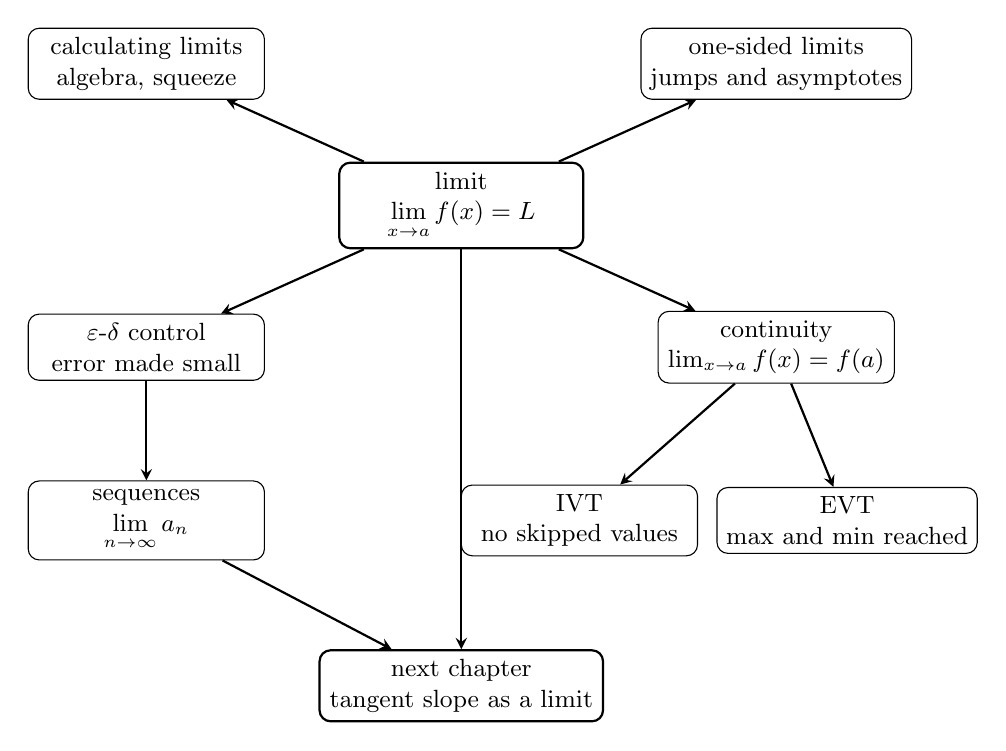
\begin{tikzpicture}[every node/.style={font=\small}, >=stealth]
  \node[draw, rounded corners, thick, align=center, minimum width=3.1cm, minimum height=0.9cm] (limit) at (0,0)
    {limit\\ \(\displaystyle \lim_{x\to a}f(x)=L\)};

  \node[draw, rounded corners, align=center, minimum width=3.0cm] (calc) at (-4,1.8)
    {calculating limits\\ algebra, squeeze};
  \node[draw, rounded corners, align=center, minimum width=3.0cm] (oneside) at (4,1.8)
    {one-sided limits\\ jumps and asymptotes};
  \node[draw, rounded corners, align=center, minimum width=3.0cm] (precise) at (-4,-1.8)
    {\(\varepsilon\)-\(\delta\) control\\ error made small};
  \node[draw, rounded corners, align=center, minimum width=3.0cm] (cont) at (4,-1.8)
    {continuity\\ \(\lim_{x\to a}f(x)=f(a)\)};

  \node[draw, rounded corners, align=center, minimum width=3.0cm] (ivt) at (1.5,-4.0)
    {IVT\\ no skipped values};
  \node[draw, rounded corners, align=center, minimum width=3.0cm] (evt) at (4.9,-4.0)
    {EVT\\ max and min reached};
  \node[draw, rounded corners, align=center, minimum width=3.0cm] (seq) at (-4,-4.0)
    {sequences\\ \(\displaystyle \lim_{n\to\infty}a_n\)};

  \node[draw, rounded corners, thick, align=center, minimum width=3.6cm, minimum height=0.9cm] (deriv) at (0,-6.1)
    {next chapter\\ tangent slope as a limit};

  \draw[->, thick] (limit) -- (calc);
  \draw[->, thick] (limit) -- (oneside);
  \draw[->, thick] (limit) -- (precise);
  \draw[->, thick] (limit) -- (cont);
  \draw[->, thick] (cont) -- (ivt);
  \draw[->, thick] (cont) -- (evt);
  \draw[->, thick] (precise) -- (seq);
  \draw[->, thick] (seq) -- (deriv);
  \draw[->, thick] (limit) -- (deriv);
\end{tikzpicture}
\caption{Limits are the center.  Continuity, asymptotes, sequences, and tangent slopes all use the same idea of controlled approach.}
\label{fig:chapter3-concept-map}
\end{figure}

The most important habit is not memorizing a table of limit forms.  It is asking:

\[
\text{What is the input doing, and what target is the output approaching?}
\]

\subsection{A decision guide for limits and continuity}
\label{subsec:chapter3-decision-guide}

When you face a limit problem, begin with the simplest test.  Then move only as far as the problem requires.

\[
\begin{array}{>{\centering\arraybackslash}p{0.35\textwidth}|p{0.58\textwidth}}
\textbf{what you see} & \textbf{what to try} \\ \hline
direct substitution gives a real number &
Use continuity or the limit laws. \\[4pt]
direct substitution gives \(\dfrac00\) &
Factor, cancel, expand, combine fractions, or rationalize.  Then try again. \\[8pt]
left and right sides behave differently &
Compute one-sided limits.  A two-sided limit exists only if they agree. \\[6pt]
denominator approaches \(0\) without cancellation &
Check signs from the left and right.  The limit may be \(\infty\), \(-\infty\), or may fail to exist. \\[6pt]
\(x\to\infty\) or \(x\to-\infty\) &
Divide by the largest power, or compare leading terms. \\[6pt]
an oscillating factor is multiplied by something small &
Try the squeeze principle. \\[6pt]
a theorem about continuous functions is tempting &
Check the hypotheses first: continuity, closed interval, bounded interval, and the right endpoint information. \\[6pt]
a sequence appears &
Use the \(\varepsilon\)-\(N\) definition, algebraic limit laws, or monotone bounded convergence.
\end{array}
\]

The warning examples in Section \ref{sec:warning-examples-limits-continuity} should stay close by.  Most mistakes come from using a true theorem without checking the conditions that make it true.

\subsection{Review problems}
\label{subsec:chapter3-review-problems}

The problems below are grouped by purpose.  Some are computational.  Some ask for explanations.  Some ask for proof.  In the proof problems, the goal is not speed.  The goal is control.

\subsubsection*{A. Concept checks}

\begin{enumerate}
\item Explain the difference between

\[
\lim_{x\to a}f(x)
\qquad\text{and}\qquad
f(a).
\]

Give an example where the limit exists but does not equal the function value.

\item Explain why the condition

\[
0<|x-a|<\delta
\]

appears in the definition of a limit.

\item What does the statement

\[
\lim_{x\to a}f(x)=\infty
\]

mean?  Why is this not convergence to a real number?

\item A table gives values of \(f(x)\) near \(x=3\), and the values appear to approach \(8\).  Why is the table useful?  Why is it not, by itself, a proof?

\item State the two-sided limit test using left-hand and right-hand limits.

\item In your own words, explain what continuity at \(a\) means.

\item Why can a removable discontinuity be repaired by changing one value, but a jump discontinuity cannot?

\item State the Intermediate Value Theorem.  Name its main hypothesis.

\item State the Extreme Value Theorem.  Explain why both words ``closed'' and ``bounded'' matter in the interval hypothesis.

\item Explain the difference between convergence of a sequence and convergence of a series.  Use the words \emph{terms} and \emph{partial sums}.
\end{enumerate}

\subsubsection*{B. Skills: compute and interpret limits}

Compute each limit if it exists as a finite real number.  If no finite two-sided limit exists, explain why.  When appropriate, give one-sided limits.

\begin{enumerate}
\item Polynomial and rational limits.

\[
\lim_{x\to4}(3x^2-5x+1),
\qquad
\lim_{x\to-2}\frac{x^2+1}{x-3},
\]

\[
\lim_{x\to0}\frac{5x^3-2x+7}{x^2+1},
\qquad
\lim_{x\to3}\frac{x^2-9}{x+1}.
\]

\item Removable discontinuities.

\[
\lim_{x\to3}\frac{x^2-9}{x-3},
\qquad
\lim_{x\to2}\frac{x^3-8}{x-2},
\]

\[
\lim_{x\to4}\frac{\sqrt{x+5}-3}{x-4},
\qquad
\lim_{x\to2}\frac{\frac1x-\frac12}{x-2}.
\]

\item Squeeze principle.

\[
\lim_{x\to0}x\sin\frac1x,
\qquad
\lim_{x\to0}x^2\cos\frac1{x^2},
\]

\[
\lim_{x\to0}|x|\sin\frac1x.
\]

For each one, write the inequalities that trap the function.

\item One-sided limits for a piecewise function.  Let

\[
F(x)=
\begin{cases}
x^2+2, & x<1,\\
4, & x=1,\\
3x, & x>1.
\end{cases}
\]

Find

\[
\lim_{x\to1^-}F(x),
\qquad
\lim_{x\to1^+}F(x),
\qquad
\lim_{x\to1}F(x),
\qquad
F(1).
\]

Is \(F\) continuous at \(1\)?

\item Another piecewise function.  Let

\[
G(x)=
\begin{cases}
2x+1, & x<2,\\
5, & x=2,\\
x^2-1, & x>2.
\end{cases}
\]

Find the left-hand limit, right-hand limit, two-sided limit, and function value at \(x=2\).  Is this a removable discontinuity, a jump discontinuity, or neither?

\item Infinite limits.

\[
\lim_{x\to3^-}\frac1{x-3},
\qquad
\lim_{x\to3^+}\frac1{x-3},
\]

\[
\lim_{x\to3}\frac1{(x-3)^2},
\qquad
\lim_{x\to2^-}\frac{x+2}{x^2-4},
\qquad
\lim_{x\to2^+}\frac{x+2}{x^2-4}.
\]

For each function, identify any vertical asymptote.

\item Limits at infinity.

\[
\lim_{x\to\infty}\frac{5x^2-x+1}{2x^2+3},
\qquad
\lim_{x\to-\infty}\frac{5x^2-x+1}{2x^2+3},
\]

\[
\lim_{x\to\infty}\frac{3x+7}{x^2+1},
\qquad
\lim_{x\to\infty}\frac{x^2+1}{x-1}.
\]

For the last function, decide whether there is a horizontal asymptote or a slant asymptote.

\item Slant asymptote.  Write

\[
\frac{x^2+3x}{x+1}
\]

in the form

\[
mx+b+\frac{r}{x+1}.
\]

Then find the slant asymptote as \(x\to\infty\) and as \(x\to-\infty\).

\item Sequence limits.

\[
\lim_{n\to\infty}\frac{3n+1}{2n-5},
\qquad
\lim_{n\to\infty}\left(1-\frac1n\right),
\]

\[
\lim_{n\to\infty}\frac{n^2+4}{5n^2-n},
\qquad
\lim_{n\to\infty}(-1)^n.
\]

Classify each sequence as convergent or divergent.

\item Monotone bounded sequences.  For each sequence, decide whether it is increasing, decreasing, bounded above, bounded below, and convergent.

\[
a_n=1-\frac1n,
\qquad
b_n=\frac1n,
\qquad
c_n=n,
\qquad
d_n=(-1)^n.
\]
\end{enumerate}

\subsubsection*{C. Reading limits from a graph}

Use Figure \ref{fig:chapter3-graph-reading-review} for the next problem.

\begin{figure}[h]
\centering
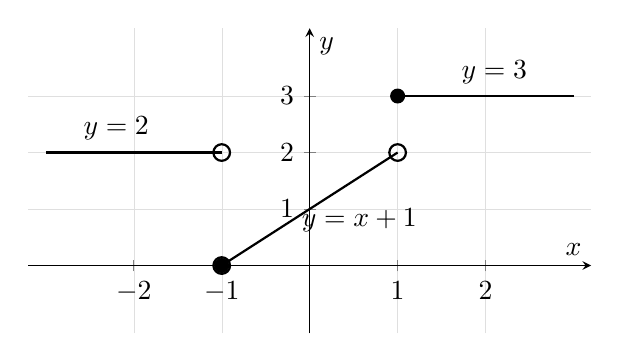
\begin{tikzpicture}
\begin{axis}[
    width=0.72\textwidth,
    height=0.45\textwidth,
    xmin=-3.2, xmax=3.2,
    ymin=-1.2, ymax=4.2,
    axis lines=middle,
    xlabel={\(x\)},
    ylabel={\(y\)},
    xtick={-2,-1,0,1,2},
    ytick={0,1,2,3},
    grid=both,
    grid style={line width=.1pt, draw=gray!25},
]
\addplot[thick, domain=-3:-1, samples=2] {2};
\addplot[thick, domain=-1:1, samples=2] {x+1};
\addplot[thick, domain=1:3, samples=2] {3};
\addplot[only marks, mark=o, mark size=3pt, thick] coordinates {(-1,2) (-1,0) (1,2)};
\addplot[only marks, mark=*, mark size=2.5pt] coordinates {(-1,0) (1,3)};
\node[anchor=south] at (axis cs:-2.2,2.05) {\(y=2\)};
\node[anchor=west] at (axis cs:-0.2,0.8) {\(y=x+1\)};
\node[anchor=south] at (axis cs:2.1,3.05) {\(y=3\)};
\end{axis}
\end{tikzpicture}
\caption{Graph for reading one-sided limits, function values, and discontinuities.}
\label{fig:chapter3-graph-reading-review}
\end{figure}

\begin{enumerate}
\item Find

\[
\lim_{x\to-1^-}f(x),
\qquad
\lim_{x\to-1^+}f(x),
\qquad
\lim_{x\to-1}f(x),
\qquad
f(-1).
\]

\item Find

\[
\lim_{x\to1^-}f(x),
\qquad
\lim_{x\to1^+}f(x),
\qquad
\lim_{x\to1}f(x),
\qquad
f(1).
\]

\item At which points shown in the graph is \(f\) discontinuous?  Classify each discontinuity as removable, jump, or neither.

\item Could changing only \(f(-1)\) make the function continuous at \(-1\)?  Explain.

\item Could changing only \(f(1)\) make the function continuous at \(1\)?  Explain.
\end{enumerate}

\subsubsection*{D. Continuity and theorem use}

\begin{enumerate}
\item Find the value of \(c\) that makes the function continuous at \(x=2\):

\[
H(x)=
\begin{cases}
x^2+c, & x<2,\\
3x-1, & x\ge2.
\end{cases}
\]

\item Find the value of \(c\) that makes the function continuous at \(x=2\):

\[
K(x)=
\begin{cases}
\dfrac{x^2-4}{x-2}, & x\neq2,\\[6pt]
c, & x=2.
\end{cases}
\]

\item Find all points where the function is discontinuous:

\[
R(x)=\frac{x+1}{x^2-1}.
\]

For each discontinuity, decide whether it is removable or infinite.

\item Use the Intermediate Value Theorem to show that the equation

\[
x^3+x-3=0
\]

has a solution in \((1,2)\).

\item Use the Intermediate Value Theorem to show that the equation

\[
x^5+x-1=0
\]

has a solution in \((0,1)\).

\item Let

\[
f(x)=x^4-4x+1.
\]

Explain why \(f\) must attain an absolute maximum and an absolute minimum on \([-2,3]\).  You do not need to find them.

\item The function

\[
f(x)=\frac1x
\]

is continuous on \((0,1)\).  Does the Extreme Value Theorem guarantee an absolute maximum and minimum on \((0,1)\)?  Explain exactly which hypothesis is missing.

\item A function \(f\) is continuous on \([0,4]\), with

\[
f(0)=-2
\qquad\text{and}\qquad
f(4)=7.
\]

What values must \(f\) take somewhere on \([0,4]\)?  What values might it take, but are not guaranteed by this information alone?

\item A function \(g\) is defined on \([0,4]\), with

\[
g(0)=-2
\qquad\text{and}\qquad
g(4)=7.
\]

But \(g\) is not continuous.  Can we conclude that \(g(c)=0\) for some \(c\in[0,4]\)?  Give an example or explain why not.

\item Give an example of a continuous function on an unbounded interval that has no absolute maximum.
\end{enumerate}

\subsubsection*{E. Proof practice with \(\varepsilon\), \(\delta\), and \(N\)}

These problems are about writing precise arguments.  Do not begin by saying ``it is obvious from the graph.''  Begin with the error you must control.

\begin{enumerate}
\item Prove from the definition that

\[
\lim_{x\to3}(2x+5)=11.
\]

\item Prove from the definition that

\[
\lim_{x\to a}(mx+b)=ma+b,
\]

where \(m\) and \(b\) are constants.

\item Prove from the definition that

\[
\lim_{x\to2}x^2=4.
\]

Hint: factor

\[
|x^2-4|=|x-2||x+2|.
\]

First make \(|x+2|\) bounded by requiring \(|x-2|<1\).

\item Prove from the definition that

\[
\lim_{x\to1}\frac{x^2-1}{x-1}=2.
\]

Remember that the definition already assumes \(x\neq1\).

\item Prove that

\[
\lim_{n\to\infty}\frac1n=0.
\]

Use the precise definition of sequence convergence.

\item Prove that

\[
\lim_{n\to\infty}\frac{2n+1}{n+3}=2.
\]

Hint:

\[
\left|\frac{2n+1}{n+3}-2\right|
=
\frac5{n+3}.
\]

\item For the sequence

\[
a_n=1-\frac1n,
\]

prove directly that \(a_n\to1\).

\item Show that the sequence

\[
b_n=(-1)^n
\]

does not converge.  Hint: if it converged to \(L\), the even terms and odd terms would both have to approach \(L\).

\item Let \(\varepsilon=10^{-4}\).  Find a value of \(N\) such that

\[
n\ge N
\quad\Longrightarrow\quad
\left|\frac1n-0\right|<10^{-4}.
\]

\item Let

\[
a_n=\frac{n}{n+1}.
\]

Find a value of \(N\) such that

\[
n\ge N
\quad\Longrightarrow\quad
|a_n-1|<0.001.
\]
\end{enumerate}

\subsection{Project: bisection method for a root}
\label{subsec:bisection-project}

The Intermediate Value Theorem proves that roots exist.  Bisection turns that proof into a numerical method.

Use

\[
p(x)=x^3-x-1.
\]

We know

\[
p(1)=-1<0
\qquad\text{and}\qquad
p(2)=5>0.
\]

Since \(p\) is continuous, the Intermediate Value Theorem guarantees at least one root in \((1,2)\).

\paragraph{The method.}
Begin with

\[
[L_0,R_0]=[1,2].
\]

At each step, compute the midpoint

\[
M_k=\frac{L_k+R_k}{2}.
\]

Then choose the half interval where the sign change remains:

\[
[L_{k+1},R_{k+1}]
=
\begin{cases}
[L_k,M_k], & p(L_k)\text{ and }p(M_k)\text{ have opposite signs},\\
[M_k,R_k], & p(M_k)\text{ and }p(R_k)\text{ have opposite signs}.
\end{cases}
\]

If \(p(M_k)=0\), the midpoint is the exact root and the process stops.

\paragraph{Part 1: complete the table.}
Use exact arithmetic or decimal approximations.  Keep at least six decimal places in the midpoint and in \(p(M_k)\).

\[
\begin{array}{c|c|c|c|c|c}
k & L_k & R_k & M_k & p(M_k) & \text{next interval} \\ \hline
0 & 1 & 2 & 1.5 & 0.875 & [1,1.5] \\
1 & 1 & 1.5 & 1.25 & -0.296875 & [1.25,1.5] \\
2 & & & & & \\
3 & & & & & \\
4 & & & & & \\
5 & & & & & \\
6 & & & & & \\
7 & & & & &
\end{array}
\]

\paragraph{Part 2: error control.}
After \(N\) completed bisections, what is the length of the interval that still contains the root?

Start with length

\[
R_0-L_0=1.
\]

After one bisection, the length is

\[
\frac12.
\]

After two bisections, the length is

\[
\frac14.
\]

Find a formula for the length after \(N\) bisections.

\paragraph{Part 3: midpoint estimate.}
If the root \(c\) lies inside \([L_N,R_N]\), and we report the midpoint

\[
M_N=\frac{L_N+R_N}{2},
\]

show that

\[
|M_N-c|\le \frac{R_N-L_N}{2}.
\]

Use this to decide how many bisections are enough to guarantee an error less than

\[
10^{-4}.
\]

\paragraph{Part 4: why continuity matters.}
Construct a function that has

\[
f(1)<0
\qquad\text{and}\qquad
f(2)>0,
\]

but has no root in \((1,2)\).  Explain which hypothesis of the Intermediate Value Theorem fails.

\paragraph{Part 5: a root without a sign change.}
The function

\[
q(x)=(x-1)^2
\]

has a root at \(x=1\), but

\[
q(0)>0
\qquad\text{and}\qquad
q(2)>0.
\]

What does this example show about bisection?  Does bisection find every root automatically?

\paragraph{Part 6: optional computing.}
Use a spreadsheet or short program to continue bisection until the interval length is less than

\[
10^{-8}.
\]

Report the final interval and midpoint.  Then graph \(p(x)\) near the root and check that the graph agrees with your numerical result.

\subsection{Discovery problems: secant slopes becoming tangent slopes}
\label{subsec:secant-slope-discovery}

The next chapter begins where this one started: with average velocity.  The only new step is that we will give the limiting slope a name.

For a function \(f\), a point \(a\), and a nonzero number \(h\), the secant slope from \(a\) to \(a+h\) is

\[
\frac{f(a+h)-f(a)}{h}.
\]

The derivative will be the limit of this quotient as \(h\to0\), when that limit exists.

The problems below let that idea appear before its definition.

\begin{enumerate}
\item Let

\[
f(x)=x^2
\qquad\text{and}\qquad
a=2.
\]

Define

\[
m_n=\frac{f\left(2+\frac1n\right)-f(2)}{\frac1n}.
\]

Compute \(m_1,m_2,m_5,m_{10}\), and find

\[
\lim_{n\to\infty}m_n.
\]

\item For the same function, define

\[
\ell_n=\frac{f\left(2-\frac1n\right)-f(2)}{-\frac1n}.
\]

Compute \(\ell_1,\ell_2,\ell_5,\ell_{10}\), and find

\[
\lim_{n\to\infty}\ell_n.
\]

Do the right-side and left-side secant slopes approach the same number?

\item Let

\[
f(x)=x^3
\qquad\text{and}\qquad
a=2.
\]

Compute

\[
\frac{f(2+h)-f(2)}{h}
\]

for \(h\neq0\), simplify, and then find the limit as \(h\to0\).

\item Let

\[
f(x)=|x|
\qquad\text{and}\qquad
a=0.
\]

Compute the secant slope for

\[
h=\frac1n
\]

and for

\[
h=-\frac1n.
\]

Do the two sequences of slopes approach the same number?

\item Based on the previous problem, explain why the graph of \(y=|x|\) should not have a tangent slope at \(x=0\).

\item Let

\[
f(x)=\frac1x
\qquad\text{and}\qquad
a=1.
\]

Compute and simplify

\[
\frac{f(1+h)-f(1)}{h}.
\]

Then find the limit as \(h\to0\).

\item Choose your own function \(f\) and point \(a\).  Compute several secant slopes using

\[
h=0.1,\quad 0.01,\quad 0.001
\]

and

\[
h=-0.1,\quad -0.01,\quad -0.001.
\]

Make a conjecture about the limiting slope at \(a\).  Then try to prove your conjecture algebraically.
\end{enumerate}

\subsection{End-of-chapter hook}
\label{subsec:chapter3-hook-to-derivative}

A limit watches a quantity approach a target.  In this chapter, the quantity might have been a function value, a sequence term, or an average velocity.

The next chapter chooses one limit and builds a new object from it:

\[
\lim_{h\to0}\frac{f(a+h)-f(a)}{h}.
\]

The numerator measures change in output.  The denominator measures change in input.  The quotient is an average rate of change.  The limit, if it exists, is the instantaneous rate of change.

That number is the derivative.
